\documentclass[10pt,twocolumn,letterpaper]{article}
\usepackage{iccv}
\usepackage{times}
\usepackage{epsfig}
\usepackage{graphicx}
\usepackage{amsmath}
\usepackage{amssymb}

\usepackage{float}
\usepackage{lipsum}
\usepackage{stfloats}
\usepackage{multicol}
\usepackage{multirow}
\usepackage{bm}
\usepackage{etoolbox}

\usepackage{array}
\usepackage{tabulary}
\usepackage[table,dvipsnames]{xcolor} % for rowcolor
\usepackage{paralist}
\usepackage{booktabs}
\usepackage{adjustbox}
\usepackage[shortlabels]{enumitem}
\usepackage{tabu} % color table rowfont

% === for table caption
\usepackage{caption}
\captionsetup[table]{format=plain,labelformat=simple,labelsep=period}%
% \usepackage{float}  % table follow text by [H]
% === for figure subcaption
\usepackage{subcaption}
\usepackage[pagebackref=true,breaklinks=true,letterpaper=true,colorlinks,bookmarks=false,citecolor=blue,linkcolor=red]{hyperref}
% \usepackage[pagebackref,breaklinks,colorlinks,bookmarks,bookmarksopen]{hyperref}
% \hypersetup{colorlinks, citecolor=ForestGreen, linkcolor=red}%teal
\usepackage{icomma} % for comma
\usepackage{arydshln}
% \usepackage{tabulary}
% \usepackage[table]{xcolor}
\newcommand\ver[1]{\rotatebox[origin=c]{90}{#1}}
\newcommand{\fl}[1]{\multicolumn{1}{c}{#1}}
\definecolor{gray}{rgb}{0.3,0.3,0.3}
\definecolor{blue}{rgb}{0,0.5,1}
\definecolor{mask_red}{rgb}{1,0,0.8}
\definecolor{green}{rgb}{0.2,1,0.2}
\definecolor{rblue}{rgb}{0,0,1}
\definecolor{lightblue}{HTML}{6495ed}
\definecolor{lightred}{HTML}{F19C99}
\newcommand{\gray}[1]{\textcolor{gray}{#1}}
\newcommand{\green}[1]{\textcolor[RGB]{96,177,87}{#1}}
\newcommand{\lightblue}[1]{\textcolor{lightblue}{#1}}
\newcommand{\fn}[1]{\footnotesize{#1}}
\newcommand{\gbf}[1]{\green{\bf{\fn{(#1)}}}}
\newcommand{\bbf}[1]{\lightblue{\bf{\fn{(#1)}}}}
\newcommand{\rbf}[1]{\gray{\bf{\fn{(#1)}}}}
\newcommand{\obf}[1]{\textcolor{orange}{\bf{\fn{(#1)}}}}
\definecolor{graytablerow}{gray}{0.6}
\newcommand{\grow}[1]{\textcolor{graytablerow}{#1}}
\newcommand{\ZJM}[1]{\textcolor{orange}{\bf{\fn{(#1)}}}}
%\newcommand{\YKL}[1]{\textcolor{red}{\bf{\fn{(#1)}}}}
\newcommand{\YKL}[1]{\textcolor{red}{#1}}
\newcommand{\WZ}[1]{\textcolor{red}{#1}}

\usepackage{tikz}
\newcommand*\circled[1]{\tikz[baseline=(char.base)]{
\node[shape=circle,fill=gray,inner sep=0.5pt] (char) {\textcolor{white}{\footnotesize \textbf{#1}}};}}

\iccvfinalcopy % *** Uncomment this line for the final submission

\def\httilde{\mbox{\tt\raisebox{-.5ex}{\symbol{126}}}}

% Pages are numbered in submission mode, and unnumbered in camera-ready
\ificcvfinal\pagestyle{empty}\fi

\begin{document}

%%%%%%%%% TITLE
%
\title{Tightly-Coupled LiDAR-Visual SLAM Based on Geometric Features\\for Mobile Agents}

\author{
Ke Cao$^1$,
~~Ruiping Liu$^1$,
~~Ze Wang$^3$,
~~Kunyu Peng$^1$,
~~Jiaming Zhang$^1$,
~~Junwei Zheng$^1$,\\
~~Zhifeng Teng$^1$,
~~Kailun Yang$^{2,}$\thanks{Corresponding author (e-mail: {\tt kailun.yang@hnu.edu.cn}).},
~~Rainer Stiefelhagen$^1$\\
\normalsize
$^1$Karlsruhe Institute of Technology,
\normalsize
~~$^2$Hunan University,
\normalsize
~~$^3$Zhejiang University
}

\maketitle
%
\ificcvfinal\thispagestyle{empty}\fi


%%%%%%%%% ABSTRACT
\begin{abstract}
The mobile robot relies on SLAM (Simultaneous Localization and Mapping) to provide autonomous navigation and task execution in complex and unknown environments. However, it is hard to develop a dedicated algorithm for mobile robots due to dynamic and challenging situations, such as poor lighting conditions and motion blur. To tackle this issue, we propose a tightly-coupled LiDAR-visual SLAM based on geometric features, which includes two sub-systems (LiDAR and monocular visual SLAM) and a fusion framework. The fusion framework associates the depth and semantics of the multi-modal geometric features to complement the visual line landmarks and to add direction optimization in Bundle Adjustment (BA). This further constrains visual odometry. On the other hand, the entire line segment detected by the visual subsystem overcomes the limitation of the LiDAR subsystem, which can only perform the local calculation for geometric features. It adjusts the direction of linear feature points and filters out outliers, leading to a higher accurate odometry system. Finally, we employ a module to detect the subsystem's operation, providing the LiDAR subsystem's output as a complementary trajectory to our system while visual subsystem tracking fails. The evaluation results on the public dataset M2DGR, gathered from ground robots across various indoor and outdoor scenarios, show that our system achieves more accurate and robust pose estimation compared to current state-of-the-art multi-modal methods.
\end{abstract}


%%%%%%%%% BODY TEXT


\section{Introduction}
\label{sec:intro}
% Nombrar las dificultades de hacer SLAM en un ambiente agrícola. Mencionar que es dificil hacer loop closing para disminuir el drift y que por lo tanto añadir GNSS es una buena alternativa.

\begin{figure}[!htbp]
    \centering
    \subfloat[\label{subfig:robot_front}]{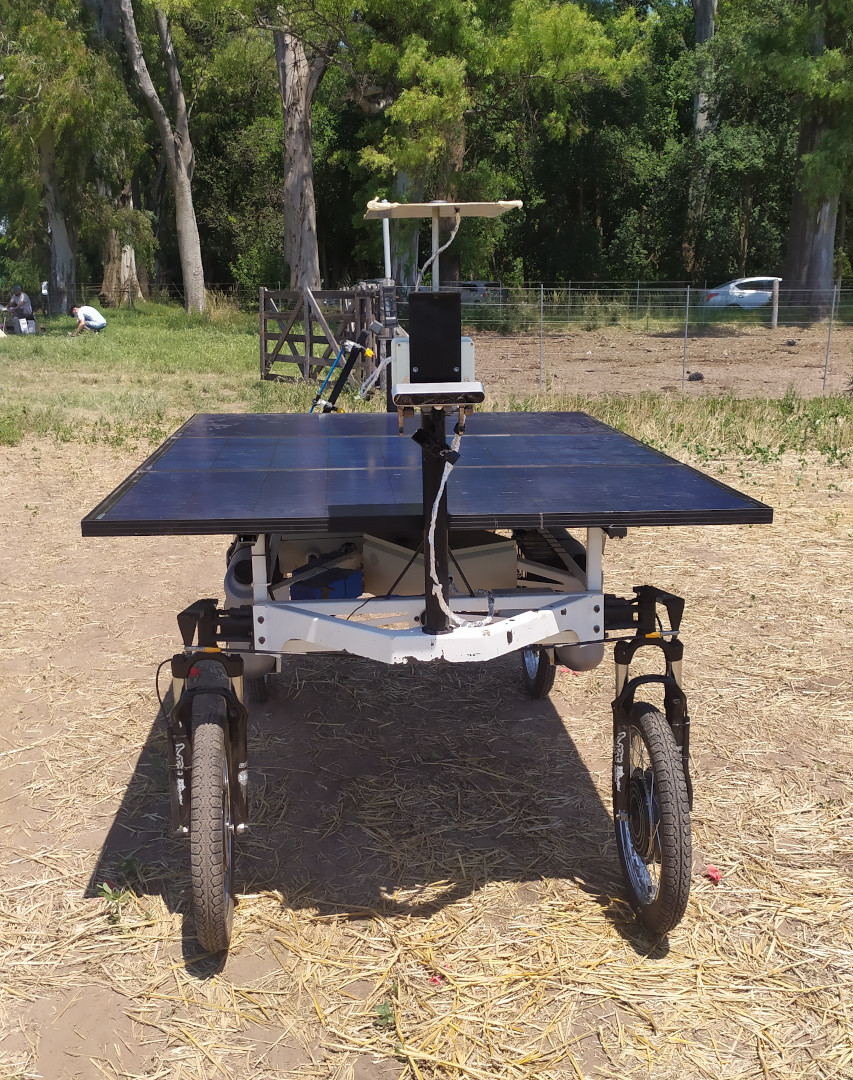
\includegraphics[width=0.4\columnwidth]{images/robot_front}}
    \hspace{0.1em}
    \subfloat[\label{subfig:robot_back}]{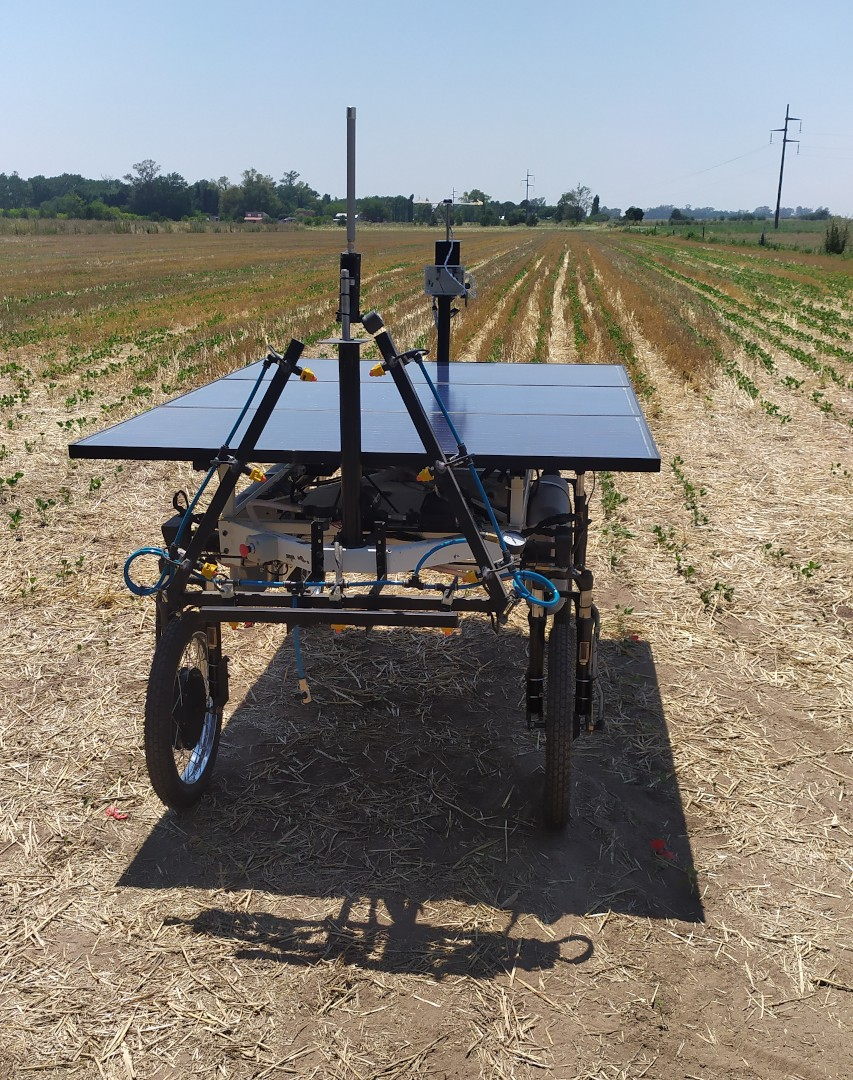
\includegraphics[width=0.4\columnwidth]{images/robot_back}}\\
    %\subfloat[]{\includegraphics[width=0.45\columnwidth]{example-image}}
    %\hspace{0.1em}
    \subfloat[\label{subfig:trajectory}]{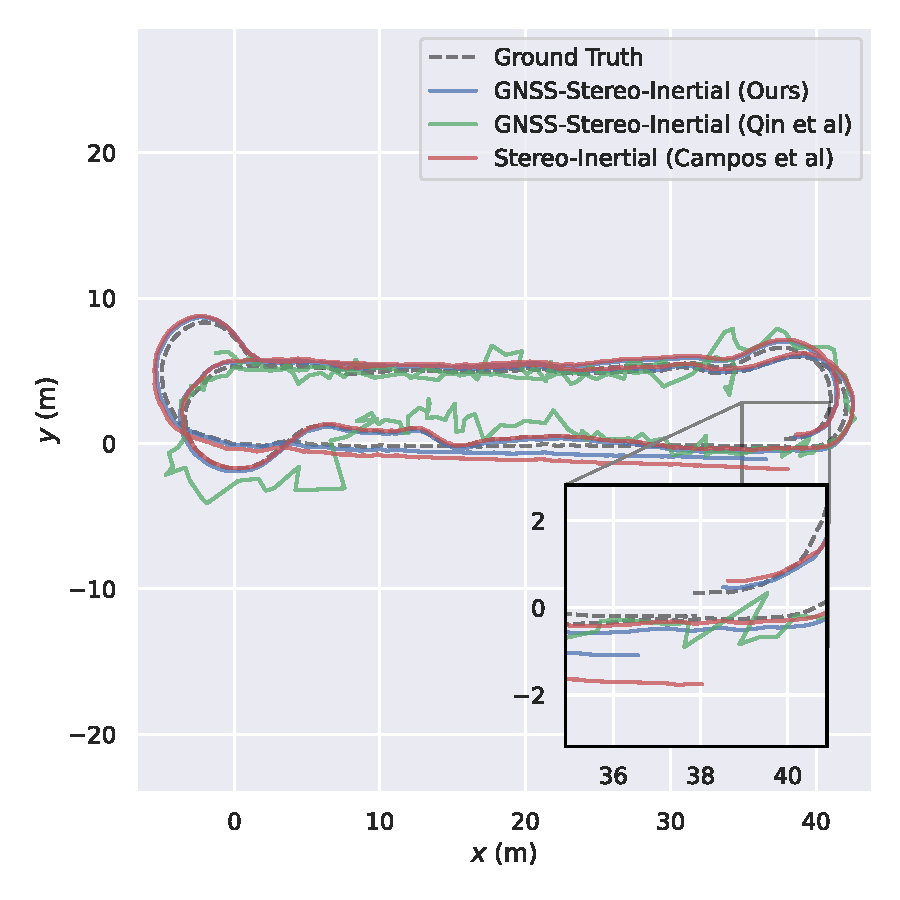
\includegraphics[width=.9\columnwidth]{images/zavalla_a.pdf}}
    \caption{\protect\subref{subfig:robot_front} and \protect\subref{subfig:robot_back}: Frontal and back views of our field robot and the arable field environment in which we navigate. \protect\subref{subfig:trajectory}: Trajectory estimated by our GNSS-stereo-inertial SLAM framework, along with GNSS-RTK ground truth,  visual-inertial ORB-SLAM3 \cite{campos2021orbslam3} and VINS-Fusion \cite{qin2019general}}
    \label{fig:teaser_image}
\end{figure}

Over the last decades, several agricultural tasks such as sowing, weed detection and removal or harvesting are being progressively automated targeting sustainable and environmentally friendly production. The use of autonomous robots in an agricultural environment has gained relevance, as it enables an efficient use of resources \cite{carelli2013agriculturalrobotics, wouter2014harvesting}. In general, in order to fully automate these and other agricultural tasks, the robot needs to know its pose relative to the environment in which it is navigating. 

A localization system must have a very high degrees of robustness and accuracy for a mobile robot to navigate safely without damaging the environment or itself. For most environments and tasks, a single sensor may not offer a sufficiently reliable robot pose estimate. As a few illustrative examples, GNSS sensors in outdoor environments do not accumulate error (drift) but they present considerable variance in their global position readings and may suffer frequent signal loss. State-of-the-art methods based on visual sensors perform badly if images have insufficient or repetitive textures, which is common in agricultural environments. Lighting can also be a problem if it is insufficient or excessive, and abrupt robot motion can cause image blur that degrades the estimation performance. Finally, interoceptive sensors that measure the internal state of the robot, such as the encoders in the wheel motors or inertial measurement units (IMU), are accurate for short-term motion estimation but drift after a few metres. Summing up, as all sensors have different and complementary advantages and disadvantages, it is essential for field robotics to properly fuse the measurements of multiple sensors to achieve robust and accurate pose estimates. This is particularly relevant to allow the robot to navigate over long periods of time (long-term navigation) and to keep the error bounded locally and globally.


SLAM, standing for Simultaneous Localization and Mapping, stands for the set of methods targeting global localization and mapping from a set of onboard sensors in a mobile agent \cite{cadena2016past}. A large number of visual-inertial SLAM pipelines have been proposed in the last decade \cite{mur2017visual,qin2018vins,campos2021orbslam3}. Many of them demonstrate high accuracy and robustness in indoor and urban environments. However, when it comes to the agricultural environment, they present problems in correctly estimating the pose of the robot. Among others, agricultural environments are challenging for visual navigation due to insufficient and/or repetitive texture and direct sunlight. Adding inertial measurements provides a slight improvement in the estimation. Nevertheless, as shown in \cite{cremona2022evaluation}, state-of-the-art visual-inertial systems accumulate significant errors after navigating a few minutes on arable lands. Robust SLAM systems such as ORB-SLAM3 \cite{campos2021orbslam3} can eliminate drift when revisiting already mapped places, but the so-called loop closing offers a poor performance on agricultural fields due to insufficiently discriminative visual appearances. A reasonable alternative, that we use in this work, is to employ measurements from global positioning sensors such as GNSS to allow the robot to navigate for long periods without accumulating drift.

This paper presents a GNSS-stereo-inertial SLAM implementation that fuses GNSS, visual and inertial measurements using a tightly-coupled approach. Specifically, we extend the state-of-the-art ORB-SLAM3 \cite{campos2021orbslam3} with GNSS factors. The global positioning measurements are incorporated into the mapping thread, so that it performs periodic corrections in the local map and hence also correct the current camera pose in the tracking thread. In this manner, we can achieve drift-less trajectories without depending on the ability of the system to close loops based on visual appearance. We evaluated our implementation on the agricultural dataset known as Rosario Dataset \cite{pire2019rosario} and an additional in-house dataset, which contains data from a wheeled robot in a soybean field (see Figure \ref{subfig:robot_front}-\ref{subfig:robot_back} for a picture of our robot). In both cases, we show how our implementations is able to effectively fuse GNSS readings outperforming the original stereo-inertial ORB-SLAM3. The contribution of the work can be summarized as follows:
\begin{itemize}
    \item Implementation of a GNSS-Stereo-Inertial framework.
    \item Evaluation of our GNSS-Stereo-Inertial framework tightly-coupled fusion in agricultural environments, incorporating real conventional GNSS measurements instead of simulated ones, which are rarely included in evaluations of state-of-the-art approaches.
    \item Public release of our implementation as open-source\footnote{\href{https://github.com/CIFASIS/gnss-stereo-inertial-fusion}{\nolinkurl{https://github.com/CIFASIS/gnss-stereo-inertial-fusion}}} , in order to facilitate its usage, extensions and comparisons and evaluations by the robotics community.
\end{itemize}

The article is organized as follows: Section~\ref{sec:related} discusses related work on multi-modal sensor fusion. In  Section~\ref{sec:method}, we describe the proposed GNSS-Stereo-Inertial framework. In Section~\ref{sec:experiments}, we present and discuss the experimental results of our GNSS-Stereo-Inertial implementation on real data in an agricultural field. Finally, we present our conclusions in Section~\ref{sec:conclusions}.


\section{Related Work}
\label{sec:related_work}
\begin{figure*}
  \centering
  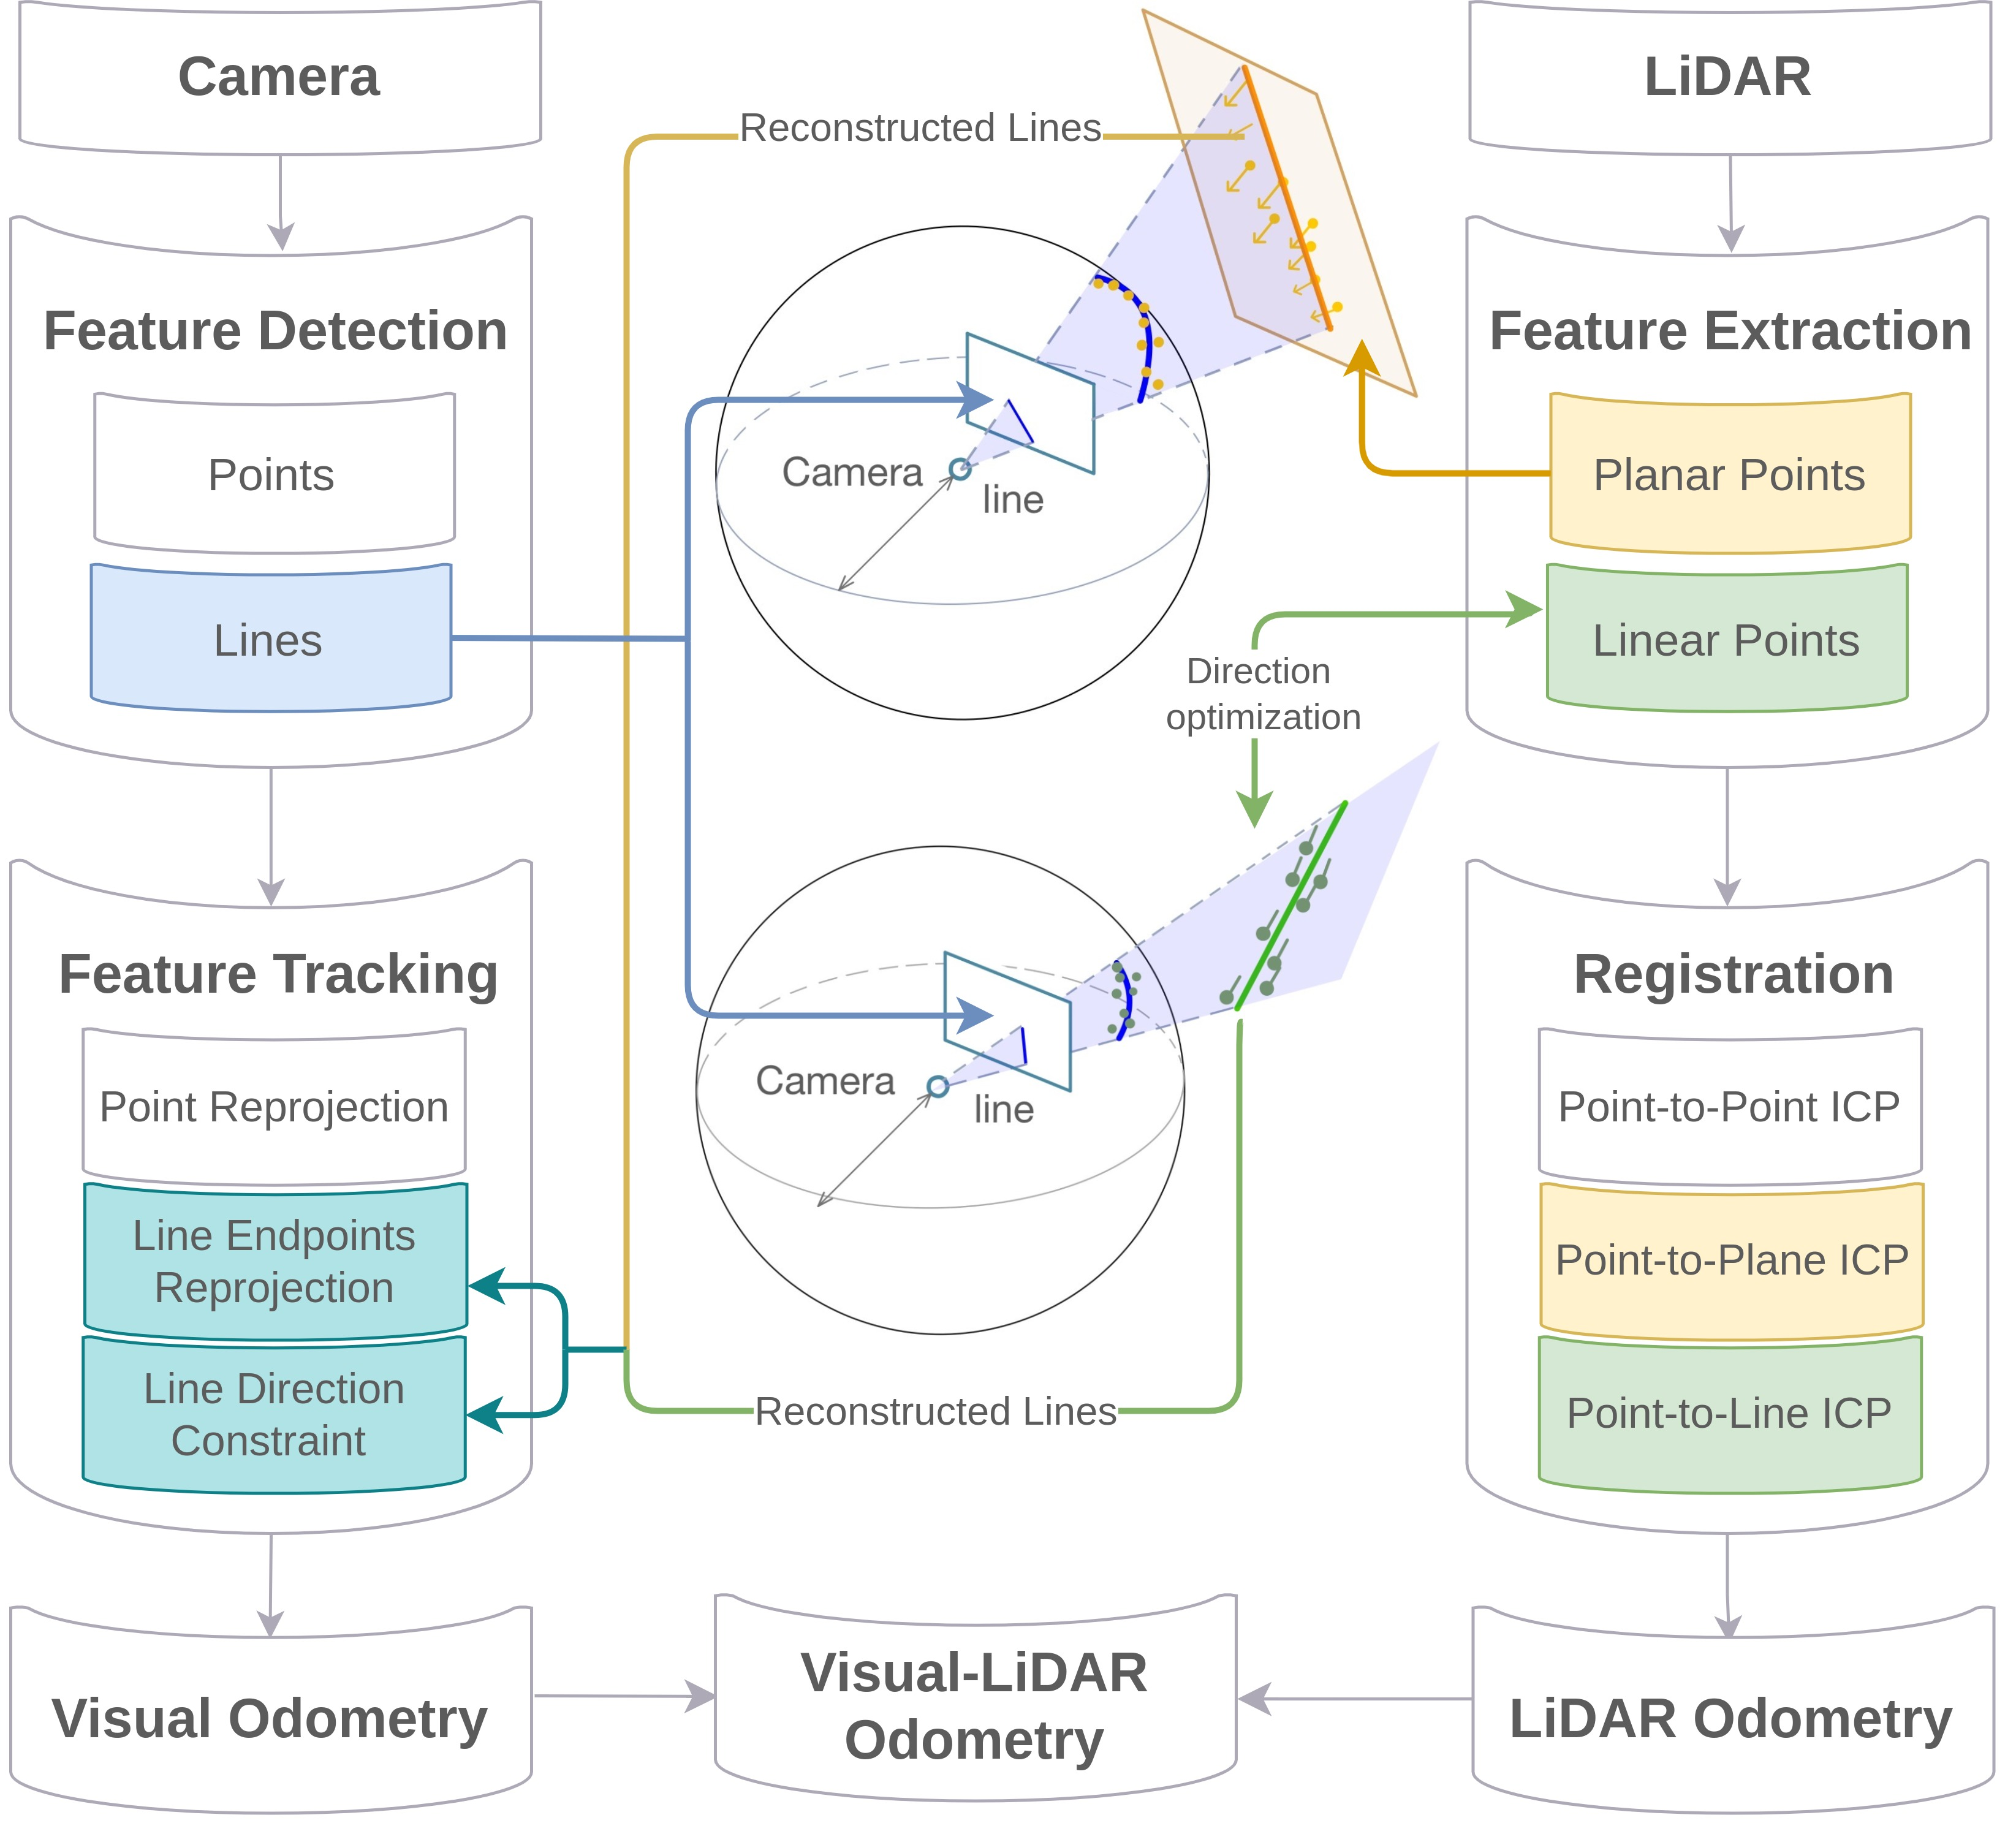
\includegraphics[width=0.62\textwidth]{images/overview.jpg}
  \caption{Overview of our multi-modal SLAM system. It consists of a fusion framework (middle section) and dual systems - the visual SLAM subsystem (left flow) and the LiDAR SLAM subsystem (right flow). The geometric features are extracted by subsystems and then passed to the fusion framework to perform the fusion computations. The generated lines are returned to the subsystems to optimize their odometry and map.} 
  \label{fig:overview}
  \vskip -3ex
\end{figure*}

\noindent\textbf{Multi-modal SLAM.}
Previous multi-modal works can be classified by the type of sensors.
Visual SLAM~\cite{campos2021orb, leutenegger2015keyframe, mur2017visual} optimizes the reprojection error and temporal error by adding other information from IMU and correcting the scales.
Filter-based algorithms~\cite{chen2018review, geneva2020openvins, mourikis2007multi} use inertial measurements for state propagation and update the visual data to improve accuracy.

In the field of high-cost and high-complexity visual-LiDAR-inertial SLAM systems, the optimization-based algorithm LVI-SAM~\cite{shan2021lvi}, consisting of two subsystems, builds on a factor graph and accomplishes tightly-coupled odometry.
TVL-SLAM~\cite{chou2021efficient} proposes a novel large-scale bundle adjustment optimization, which compresses the LiDAR and visual residuals to achieve real-time performance in the degraded environment.
Extended Kalman Filter (EKF) based algorithms~\cite{lin2022r,lin2021r,zuo2019lic,zuo2020lic} contribute to enhancing robustness in environments with weak texture or even no features.

The visual-LiDAR SLAM systems~\cite{seo2019tight, shin2020dvl, zhang2015visual} provide a low-cost, low-compute, high-precision method for mapping and calculating odometry.
DEMO~\cite{zhang2014real, zhang2017real} is the first to associate LiDAR depth measurements with Harris corner features.
However, due to the lack of loop closure, the accumulated residuals cannot be optimized and eliminated.
Liang~\etal~\cite{liang2016visual} address this issue by proposing a scan-matching method with a visual loop detection scheme using ORB features~\cite{rublee2011orb} and a Bag-of-Words model. 

However, the extracted point-only depth as prior factors has a flaw: The multi-sensor aligned error caused by mechanical changes cannot be mitigated without an automatic extrinsic calibration procedure.
LIMO~\cite{graeter2018limo} projects the point cloud onto the image and estimates the point depth by a subset of points within a fixed rectangular region around it. To minimize the number of outliers, a filtering mechanism was introduced. This mechanism limits the depth estimation to subsets within planes.
Huang~\etal~\cite{huang2020LiDAR} explore prior structural information for point-line Bundle Adjustment (BA) and create a novel scale correction scheme.
Although it reduces the system's sensitivity to noise and motion blur, LiDAR-enhanced visual odometry becomes more challenging in underexposed scenarios.
Differing from existing works, our approach is unique in that we incorporate LiDAR-enhanced visual odometry while also developing visual-enhanced LiDAR odometry. This method is designed to be more robust in undesirable lighting conditions.

\noindent\textbf{Line-based SLAM.}
Line-based SLAM performs robustly in man-made scenes, especially when point features are sparse or unevenly distributed in images.
Its map exhibits remarkable richness, comprising a diverse range of geometric elements. Therefore, feature-based and direct visual SLAM systems incorporate geometric features to enhance localization accuracy and robustness in scenes with weak textures and lighting variations.
Visual SLAM~\cite{ram2021rp,  shu2022structure, zhang2020plane}, incorporating plane features, increases the computational complexity of feature extraction and matching.

Feature-based methods~\cite{gee2006real, gomez2019pl, pumarola2017pl, smith2006real} use traditional line detection algorithms like LSD~\cite{engel2014lsd} and perform descriptor-based tracking by minimizing the line projection.
Since the line has only four Degrees of Freedom (DoF), the two-endpoints representation line introduces six parameters, resulting in overparameterization.
Bartoli and Adrien~\cite{bartoli2005structure} propose an orthogonal representation that uses a three-DoF rotation matrix and a one-DoF rotation matrix to update line parameters during optimization.

Lines determined by two-view triangulation often occur during subsequent tracking, which wastes computational resources for detecting, describing, and matching line features.
Problems like line degeneracy occur more frequently when it is close to the epipole.
Lee~\etal~\cite{lee2019elaborate} suggests reconstructing the line segments with multiple views instead of just two.
Furthermore, several algorithms~\cite{lim2021avoiding, yang2019visual} investigate different scenarios of degenerate motion.
They modify LSD and set additional parameters to extract discernable long-line features to prevent this degeneration.

Many visual SLAMs~\cite{georgis2022vp, lee2021plf, lim2022uv, wang2021vanishing} extract vanishing points to add constraints associated with parallel 3D lines to optimize robot pose estimation.
In addition, the PLF-VINS algorithm~\cite{lee2021plf} also integrates point-line coupling residuals based on the similarity of corner points and line features.
This integration ensures accurate depth estimation.

Line-based visual SLAM is commonly used in man-made indoor scenes. Unlike existing works, our approach stands out by combining the accurate geometric features of a LiDAR point cloud with the overall structural information from an image. This results in more effective utilization of line features in a wider range of scenarios.




\section{Methodology}
\label{sec:methodology}
\subsection{System Overview}

The flowchart of the proposed multi-modal system is shown in Figure~\ref{fig:overview}, which contains the hardware and software frameworks.
The hardware framework consists of a pinhole camera and a solid-state multi-beam LiDAR sensor.
The popular and consumer-grade RGB camera serves as an efficient sensor for the robot agent due to its high performance. The LiDAR sensor captures a comprehensive $360${\textdegree} horizontal surround view of the environment, providing stable depth information even in challenging real-world scenarios. Its long-range capabilities make it well-suited for outdoor usage.
%

The software framework, a tightly-coupled multi-modal SLAM system, comprises four primary modules: a fusion framework, a detection module, and two subsystems, \ie, the LiDAR SLAM system and the monocular visual SLAM system.
These subsystems perform odometry estimation and mapping tasks independently while exchanging geometric information. 

\begin{figure}
  \centering
  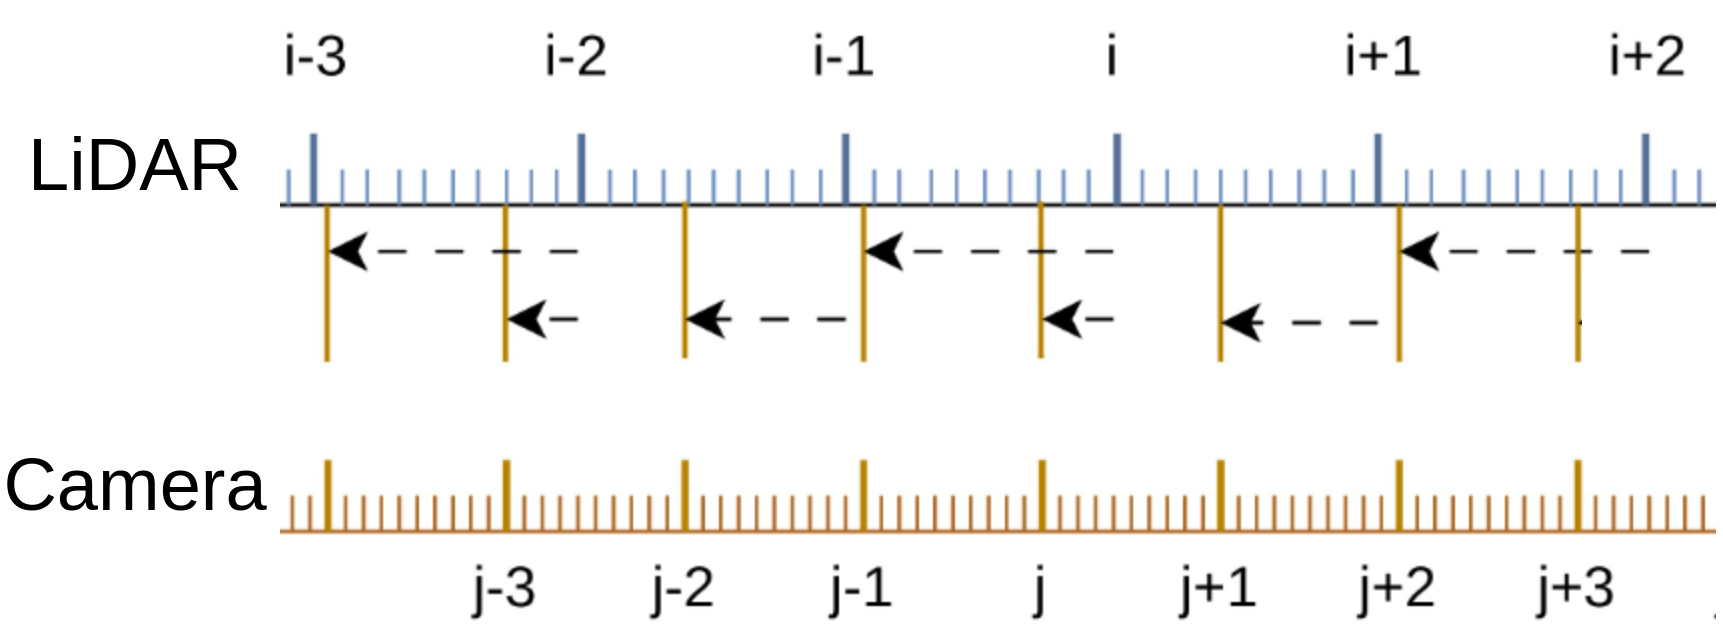
\includegraphics[width=0.42\textwidth]{images/timestamp_m.png}
  \caption{LiDAR sensor data is aligned to the camera timestamp for temporal consistency.}
  \label{fig:timestamp}
  \vskip -3ex
\end{figure}

After receiving sensor data, each subsystem proceeds to extract geometric features. The visual system utilizes ORB~\cite{rublee2011orb} and LSD~\cite{engel2014lsd} algorithms to detect points and lines in images. On the other hand, the LiDAR system employs PCA algorithm~\cite{hackel2016fast, weinmann2013feature} to extract point, linear, and planar features. To overcome the limitations imposed by individual sensor types, the fusion framework 
%
combines the geometric features and projects them into spherical coordinates, creating a unified representation that incorporates both temporal and spatial dimensions. By performing a K-D tree search, we establish a definitive correlation between the detected lines and the depths of geometric features in the point cloud. This correlation allows us to reconstruct depth measurements for line segments that cannot be accurately triangulated by the visual subsystem alone.

Once reconstructed by the fusion framework, the lines serve as new features with precise depth and are fed back to the subsystems for motion estimation and optimization. In the LiDAR subsystem, the linear directions along the same line can be inconsistent due to sparse point clouds. 
%
The fusion framework determines their average direction, which is used to adjust the directions of the linear features in the LiDAR subsystem, reducing the occurrence of outliers. When both the fusion framework's data association and the visual subsystem's triangulation provide the direction of the same line segment, the visual subsystem introduces a new optimization term called the ``line direction residual''. This term evaluates the angular difference between the two directions. By iteratively minimizing this residual, the system effectively constrains the direction of the line landmarks.

Our system relies on the visual subsystem's output to determine its odometry, which exhibits higher precision in scenes with abundant texture. However, given the increased likelihood of visual SLAM tracking failure, we incorporate a detection module to verify the proper functioning of the visual subsystem. In cases where the visual module fails, the system seamlessly switches to the more reliable LiDAR subsystem to perform pose estimation. This crucial capability ensures enhanced robustness, enabling the system to maintain accurate localization and mapping even in challenging scenarios.

\subsection{Fusion Framework}
\noindent\textbf{Preprocessing - temporal and spatial alignment.} The integration of sparse geometric features from sensors with varying positions and frequencies inherently poses challenges within the unaligned fusion framework. We employ data accumulation and temporal and spatial consistency, enhancing the reliability of our approach effectively.

By accumulating multi-frame point clouds, our system achieves a higher level of detail in the point cloud, comparable to that of the camera image.  This increased resolution allows easier matching of geometric features between the point cloud and the camera image.

Figure \ref{fig:ground_robot} demonstrates that the camera and LiDAR sensors are mounted at different angles and positions. To integrate data from both sensors into a unified coordinate system, we leverage extrinsic calibration. This calibration provides the necessary information about the relative transformation between the camera and LiDAR, enabling accurate alignment of data acquired from both sensors.

To maintain temporal consistency, it is crucial to synchronize data between LiDAR and the camera. We define the camera coordinate system and timestamp as the reference. As illustrated in Figure~\ref{fig:timestamp}, we align the LiDAR point cloud within the time interval from frame $j$ to $j+1$ to the timestamp $t_{j+1}$. During each sweep, we calculate the time difference from each point to the end of the sweep period $t_{j+1}$. Assuming a constant angular and linear velocity over this short period and that the initial pose remains the same as the previous frame, we employ linear interpolation to compute the relative pose for each point and project it onto the timestamp $t_{j+1}$. This process achieves temporal consistency within our system.

\noindent\textbf{Depth and direction association of geometric features.} After achieving spatial and temporal alignment, the geometric features from both subsystems are projected onto a spherical coordinate system centered at the camera. This projection is illustrated in Figure~\ref{fig:arc}, where a 2D visual line segment is projected onto the sphere as an arc. To perform the subsequent neighborhood search, we need to discretize the arcs and ensure a consistent density. To achieve this, we uniformly sample the arc at regular intervals $\Delta \varphi$ by incrementing the angle and determining the corresponding positions of the sampled points.
This sampling process results in a set of points along the arc with uniform spacing.
To process the LiDAR information, we first project the dense geometric point cloud onto a sphere. We then store all LiDAR geometric feature points in a 3D KD-tree~\cite{mark2008computational} and search for the closest geometric neighbor of each point along the visual arc. This iterative process continues until all points along the arc are successfully matched with their corresponding LiDAR feature points. This robust relationship between the visual arc and the LiDAR feature points allows for accurate line reconstruction. 

In the visual frame, we utilize the Line Segment Detector (LSD) algorithm to detect line features by identifying pixel regions with significant gradient changes. The first type comprises lines present on smooth surfaces, \textit{e.g.}, door or window frames. These features are extracted as planar features within the LiDAR point cloud. The second type encompasses linear features, including boundaries between different surfaces or well-defined linear elements, \textit{e.g.}, wall-floor boundaries, or trees. These characteristics are identified as linear features within the LiDAR point cloud.

\begin{figure}
  \centering
  \begin{subfigure}{0.47\linewidth}
    \centering
    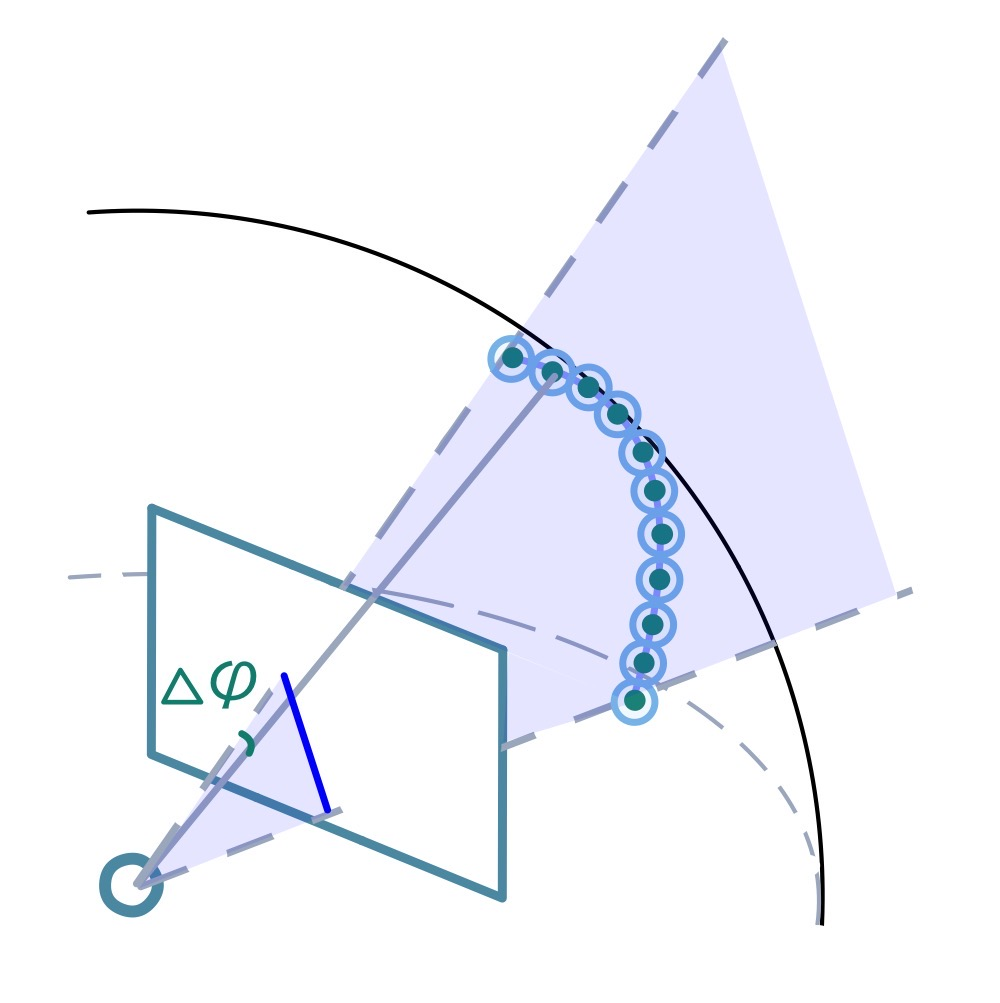
\includegraphics[width=\linewidth]{images/arc_sphere.jpg}
    \caption{Decomposition of the arc into points}
    \label{fig:arc}
  \end{subfigure}
  \hfill
  \begin{subfigure}{0.47\linewidth}
    \centering
    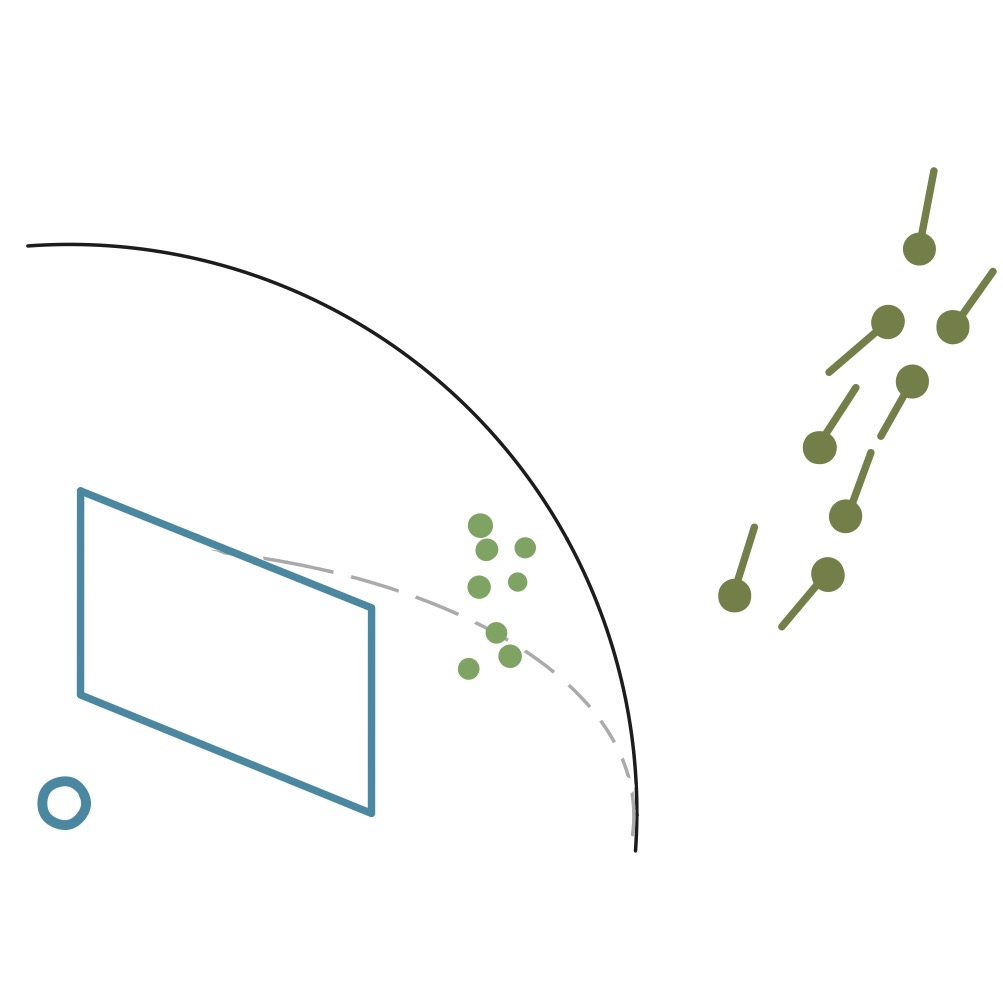
\includegraphics[width=\linewidth]{images/lidar_bad_direction.jpg}
    \caption{Direction of LiDAR linear points before optimization}
    \label{fig:lidar_bad_direction}
  \end{subfigure}

  \vskip -3ex

  \begin{subfigure}{0.47\linewidth}
    \centering
    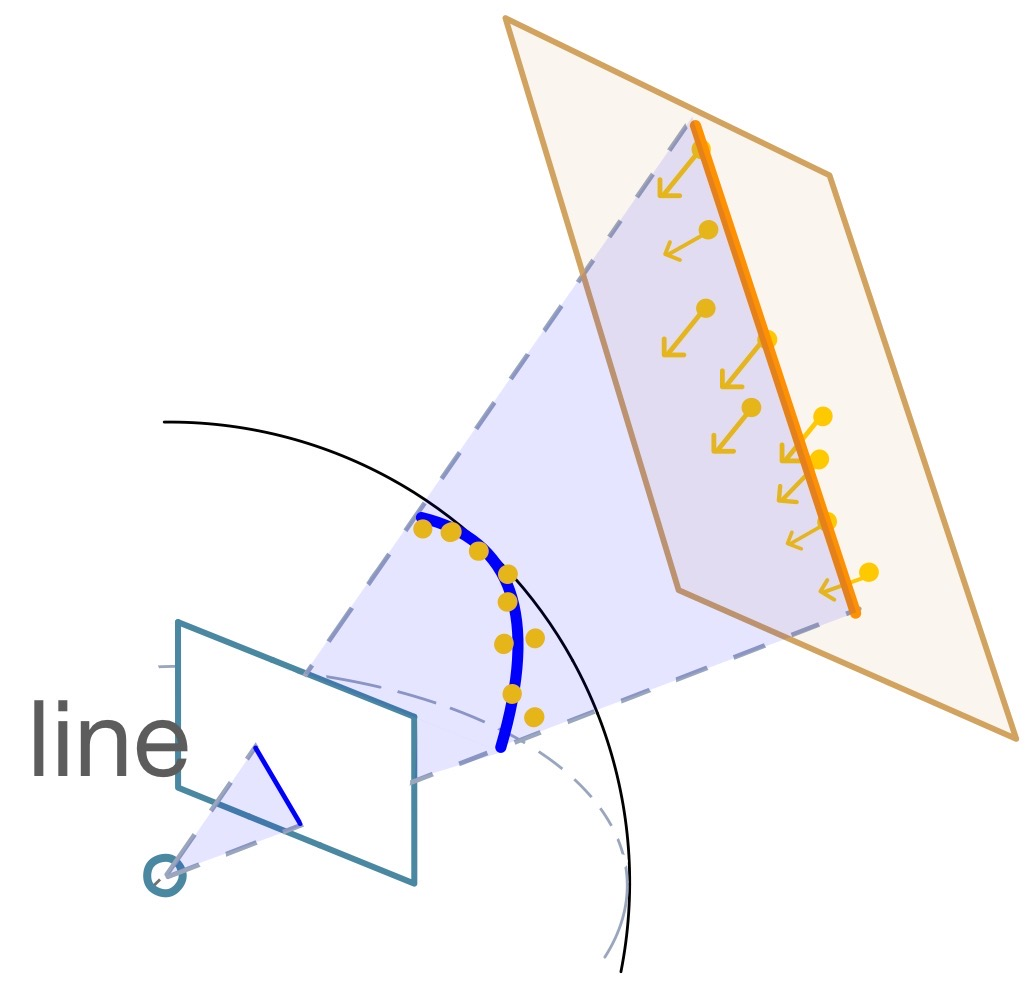
\includegraphics[width=\linewidth]{images/fusion_surface.jpg}
    \caption{Reconstruction line based on LiDAR planar features}
    \label{fig:linear_reconst}
  \end{subfigure}
  \hfill
  \begin{subfigure}{0.47\linewidth}
    \centering
    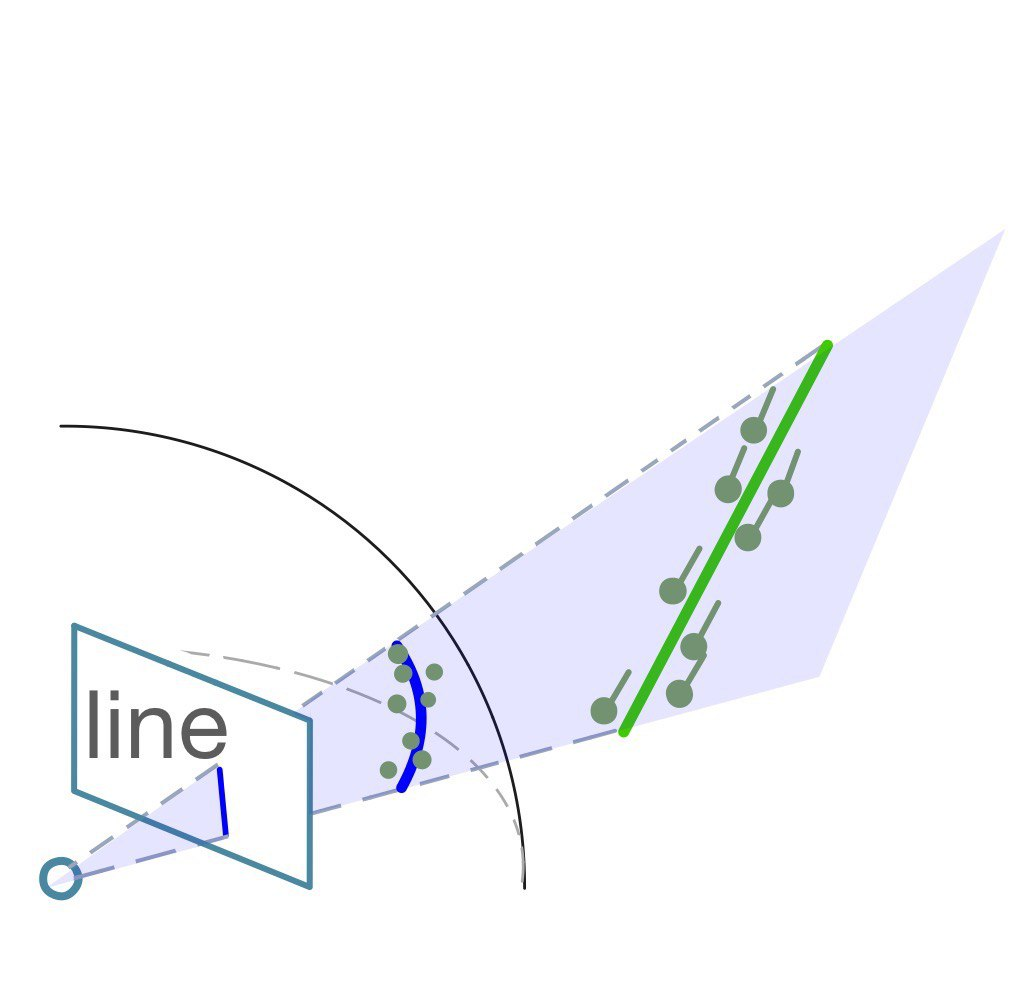
\includegraphics[width=\linewidth]{images/fusion_linear.jpeg}
    \caption{Reconstruction line based on LiDAR linear features}
    \label{fig:planar_reconst}
  \end{subfigure}

  \caption{Processing in the fusion framework.}
  \label{fig:four_images}
  \vskip -3ex
\end{figure}

Therefore, we divide the reconstruction lines, \textit{i.e.}, fusion lines, into two cases. When the majority of the surrounding point cloud comprises planar features, we utilize a plane-to-plane intersection approach to determine the fusion line, as depicted in Figure~\ref{fig:linear_reconst}. Firstly, we reconstruct a virtual LiDAR surface by utilizing appropriate planar feature points and their normal vectors. Subsequently, we project the arc into three-dimensional space, obtaining a projected plane. This plane is then intersected with the LiDAR plane to construct the fusion line.

Alternatively, if the visual arc, as illustrated in Figure~\ref{fig:planar_reconst}, is surrounded by multiple linear features, the points $L_s$ are considered as part of a single line. We select clusters that exhibit similar directions to compute the average line direction, denoted as $L_{best}$. With a point and direction on a line, we determine the line segment based on these linear points.

The fusion frame establishes a spherical coordination system to effectively integrate features from multiple modalities. Under spatiotemporal consistency, the fusion process generates additional lines that are then fed back to the respective subsystems for more accurate localization and mapping.

\subsection{Visual Subsystem}
Our visual subsystem, a derivative of Structure PLP~\cite{shu2022structure}, performs visual SLAM by tracking feature points and feature lines. It comprises three distinct modules, \textit{i.e.}, the line extraction, the line reconstruction, and the joint optimization. Each module leverages information from the visual subsystem and fusion framework to modify and filter out inaccurate data, and assist in pose optimization. 
%

\noindent\textbf{Line detection.} During the feature extraction, we utilize the LSD~\cite{engel2014lsd} algorithm to detect line segments. To enhance the performance of LSD, we refine hidden parameters and implement length rejection, following the methodology of Structure PLP~\cite{shu2022structure}. These modifications contribute to improving the computational efficiency and accuracy of our visual system during feature extraction.

\noindent\textbf{Line reconstruction with triangulation} To reconstruct the detected lines in 3D space, we utilize two methods. The first method involves triangulating the matched line segments across two frames. By using the observed endpoints ${x_s, x_e}$ of a line segment $z$, we calculate the line vector ${l} = {x}_s \times {x}_e$. Using the camera projection matrix $P\in \mathbb{R}^{3 \times 4}$, which only contains the intrinsic camera parameters, we project the observed 2D line onto the camera coordinate system. This projection results in the projection plane $\pi_i = {l}_i^{\top} \mathrm{P}_i$.

The intersection of the two projection planes $\pi_1$ and $\pi_2$ forms a 3D line in world coordinates. We represent this line using the Plücker coordinate system, denoted as $\mathbf{L}=\left(\mathbf{m}^{\top}, \mathbf{d}^{\top}\right)^{\top}$. To obtain its dual Plücker matrix $L^*_w$, the following calculation is performed:
\begin{equation}
\mathrm{L^*_w}=\pi_{1}\pi_{2}^{\mathrm{T}}-\pi_{2}\pi_{1}^{\mathrm{T}}\in\mathbb{R}^{4\times4}
\end{equation}

If the line cannot be successfully triangulated but is provided by the fusion framework, we need to convert this line segment from the Cartesian coordinate system to the Plücker coordinate system. 

Given two endpoints of the 3D lines $\overline{\mathbf{A}}$  and $\overline{\mathbf{B}}$, it is deduced that $\mathbf{L}=\left(\mathbf{m}^{\top}, \mathbf{d}^{\top}\right)^{\top}$ with
\begin{equation}
\left\{\begin{array}{l}
\mathbf{m}=\overline{\mathbf{A}} \times \overline{\mathbf{B}} \\
\mathbf{d}=\overline{\mathbf{B}}-\overline{\mathbf{A}}
\end{array}\right.
\end{equation}

\noindent\textbf{Endpoints trimming.} Line landmarks may have errors due to triangulation using only two frames. Similarly, line reconstruction in fusion frames can suffer from inaccuracies, particularly due to potential imperfections in the spatio-temporal alignment of two-sensor data. Therefore, we refine the endpoints with the method proposed in \cite{lee2019elaborate, zhang2015building}. 

In Structure PLP, endpoint trimming is utilized in local bundle adjustment (LBA). After this trimming, a depth check is performed with a threshold ratio of $0.1$ to filter out outliers based on the median depth change ratio of the scene. Considering the higher confidence in lines from the fusion framework, the outlier rejection threshold is set to $0.2$ for fusion line segments. 
%

\noindent\textbf{Endpoints re-projection and direction residual of line.} Once the observed line segment is detected, we calculate the distances between the endpoints $x_s$ and $x_e$ of the observed line segment $z$ and the projected line segment $l'$. The residual of the line measurement model is defined as the following reprojection error:
\begin{equation}
e_{dis}=d(z,l')=\begin{bmatrix}
\frac{\mathbf x_s^\top \mathbf l'}{\sqrt{l_1^{2}+ l_2^{2}} }   & \frac{\mathbf x_e^\top \mathbf l'}{\sqrt{l_1^{2}+ l_2^{2}} }
\end{bmatrix}^\top
\end{equation}

Many visual SLAM systems that use line features focus primarily on optimizing endpoints while ignoring their directions. Due to the considerable length of fusion line segments, their direction tends to be reliable. We introduce a new type of optimization, called ``line direction optimization'', which imposes additional constraints on the direction of line landmarks.

In our method, we compare the direction $\mathbf d_{fu}$ of the fusion line with the reconstructed line direction $\mathbf d_{cam}$ obtained from the visual subsystem. We unitize the two direction vectors and introduce an additional optimization term to measure the angle between these unit vectors:
\begin{equation}
\begin{aligned}
e_{dir}&=1-\cos (\mathbf d_{cam}, \mathbf d_{fu}) \\
& = 1 -
\frac{\mathbf d_{cam}^\top \mathbf d_{fu}}{\sqrt{d_{cam1}^{2}+ d_{cam2}^{2}} \sqrt{d_{fu1}^{2}+ d_{fu2}^{2}} }
\end{aligned}
\end{equation}

Considering the increasing gradient of this error term with larger errors, we incorporate a robust cost function. This effectively mitigates the influence of outliers, improving the overall stability of the optimization process. 
Moreover, since the angle measurement is independent of the image pyramid level, there is no need to introduce an information matrix.

\begin{figure}
  \centering
  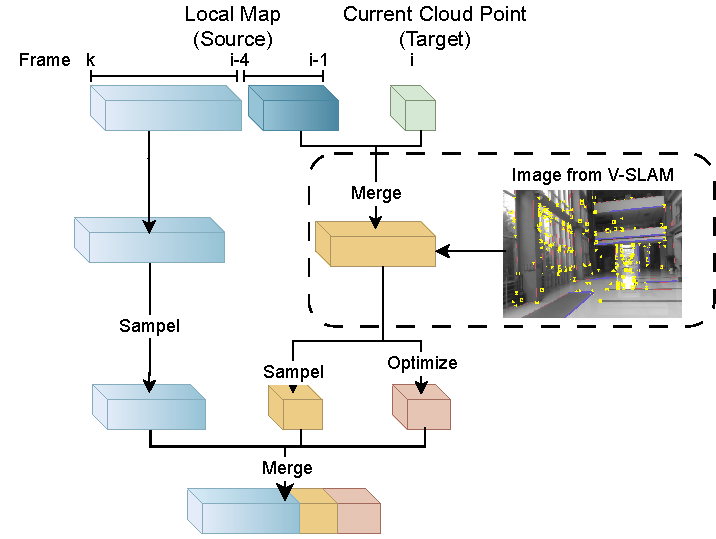
\includegraphics[width=0.5\textwidth]{images/local_map.pdf}
  \caption{An overview regarding the local map update for ICP. The point cloud of the last four frames and the current frame participate in the fusion process with the visual subsystem. The optimized point cloud is kept or sampled less. The unoptimized point clouds are downsampled. Finally, all point clouds are merged to update the local map.}
  \label{fig:local_map}
  \vskip -3ex
\end{figure}

\subsection{LiDAR Subsystem}
Following on the LiDAR SLAM MULLS~\cite{pan2021mulls}, we propose modifications to optimize our LiDAR subsystem. 
%

\noindent\textbf{Modification of the linear direction.} The geometric characteristics of each point are analyzed using the Principal Component Analysis (PCA) algorithm~\cite{hackel2016fast, weinmann2013feature}. PCA determines the local neighborhood of a point and computes the eigenvalues $\lambda_{1} \geq \lambda_{2} \geq \lambda_{3} \geq 0$ and their corresponding eigenvectors $\mathbf{e}_{1}, \mathbf{e}_{2}, \mathbf{e}_{3}$. Following these methods~\cite{hackel2016fast, weinmann2013feature}, we classify points as either linear or planar based on their one-dimensional (1D) linear structure $L_{\lambda}=\frac{\lambda_{1}-\lambda_{2}}{\lambda_{1}}$, two-dimensional (2D) planar structure $P_{\lambda}=\frac{\lambda_{2}-\lambda_{3}}{\lambda_{1}}$, and curvature measurements $C_{\lambda}=\frac{\lambda_{3}}{\lambda_{1}+\lambda_{2}+\lambda_{3}}$. 
%
The geometric features are categorized into five types: vertex, pillar, beam, facade, and roof. 

In the PCA, the size of the local neighborhood is typically limited. This limitation poses challenges in larger scenes where the structural analysis may not be fully exploited. As depicted in Figure~\ref{fig:lidar_bad_direction}, the calculated line directions along the same line exhibit slight variations. These errors have a negative impact on the point-to-line alignment within the Iterative Closest Point (ICP) process. So we leverage detected complete lines in our visual subsystem to gain a more comprehensive understanding of the line structures in the environment. Following the fusion process, we determine which LiDAR linear points ($L_s$) belong to the same line with a consistent line direction. This association allows us to group related linear points together. Then, in the fusion framework, we calculate the mean direction ($\mathbf d_{v\_mean}$) of these lines and update the direction of all linear points by assigning them the calculated mean direction ($\mathbf d_{v\_mean}$).

\noindent\textbf{Improved storage of fusion-enhanced point cloud.} After performing the Iterative Closest Point (ICP) algorithm~\cite{besl1992method}, the target cloud must be updated for the next frame. MULLS merges and downsamples multiple historical frames into the local map. During this process, it is essential to synchronize the point clouds from different timestamps to the current timestamp $i$. This synchronization ensures that the point clouds are correctly aligned and accurately represent the environment. Although the denser local map provides a more comprehensive representation of the environment structure, merging too many historical frames means that the local map has to perform multiple alignments with the estimated pose, which leads to error accumulation. 

In order to strike a balance between preserving important geometric features and minimizing the accumulation of historical frames, a series of steps are employed in our method. As shown in Figure \ref{fig:local_map}, we combine the point cloud from the last four frames with the current frame. These point clouds are then projected onto a sphere to optimize the directions of their linear features. The optimized feature points increase the convergence speed of the ICP and improve the accuracy of the estimated values. Once the point cloud is optimized, we proceed to sample and merge them. To control the density of the local map, we introduce a threshold parameter $\alpha$ that represents the maximum rate of optimized features allowed in the local map. If the current rate of optimized points does not exceed $\alpha$, no sampling is performed. If the rate surpasses the threshold $\alpha$, we downsample the point cloud to reduce the rate until it falls below the specified threshold. Finally, the local map is updated by merging all the point clouds together.

\section{Experiments}
\label{sec:experiments}
This section shows the experimental results of the implementation proposed in Section~\ref{sec:method}. The framework is evaluated on the Rosario Dataset \cite{pire2019rosario}, a set of agricultural data captured by a weed removal robot. Later, an evaluation of the system in a soybean field is presented, using the same weed removal robot. The difference between the latter test and the evaluation on the Rosario Dataset is that new sensors are available, including measurements from a conventional GNSS.

\subsection{Rosario Dataset}
\label{sec:experiments_rosario_dataset}
The Rosario Dataset \cite{pire2019rosario} is a set of data captured by the sensors of a weed removal robot developed by the CIFASIS institute (CONICET-UNR) in Rosario, Argentina. It is composed of six sequences captured in a soybean field. The sequences contain stereo images of $672\times\SI{376}{\px}$ captured at \SI{15}{\hertz}, measurements from an IMU with a frequency of \SI{142}{\hertz} including gyroscope and accelerometer, wheel odometry obtained at \SI{10}{\hertz} and GNSS-RTK measurements at \SI{5}{\hertz}. The GNSS-RTK data are used as positional ground‐truth.

Since the Rosario Dataset does not have conventional GNSS measurements, we simulate noisy GNSS measurements by corrupting the ground-truth with zero-mean Gaussian noise, as in \cite{cioffi2020tightly}. We use isotropic Gaussian noise $\mathbf{n}_{p}\sim\mathcal{N}\left(\mathbf{0},\sigma_{p}^{2}\cdot\mathbf{I}\right)$, with a standard deviation $\sigma_{p} = \SI{0.5}{\meter}$. We selected this value from observing the covariance of the conventional GNSS used in the experiments in Section~\ref{sec:experiments_conventional_gps}. 

\begin{table}[!tp]
    \centering
    \caption{Mean and standard deviation (between parentheses) of the Absolute Trajectory Error (ATE) [\si{\metre}] for stereo-inertial ORB-SLAM3 \cite{campos2021orbslam3}, a loosely-coupled GNSS-stereo-inertial system \cite{qin2019general} and our tightly-coupled GNSS-stereo-inertial framework in the six sequences of the Rosario Dataset. Best results are in \bf{bold}.}
    
    \resizebox{\linewidth}{!} {
        \begin{tabular}{cccc}
        \hline
                    Sequence & Stereo-Inertial & GNSS-Stereo-Inertial & GNSS-Stereo-Inertial \\
                    & \cite{campos2021orbslam3} & \cite{qin2019general} & (Ours) \\
                    \hline
        01 &  0.90 (0.34)                  &
        1.44 (2.06) &
        \bf{0.86 (0.26)}                \\
        02 &  1.33 (0.75)                  &        \bf{0.90 (0.40)} &
        0.94 (0.56)                 \\
        03 &  1.12 (0.65)                  & 1.34 (1.91) & \bf{0.99 (0.56)}                \\
        04 & 1.09 (0.65)                   & 1.42 (1.20) &
        \bf{1.04 (0.60)}                \\
        05 &  0.89 (0.55)                  & 1.43 (1.91) & \bf{0.76 (0.38)}                \\
        06 & 2.48 (1.40)                   & 1.81 (0.87) &  \bf{1.23 (0.70)}     \\ \hline
        \end{tabular}
    }
    \label{tab:rosario_results}
\end{table}

We compared our GNSS-Stereo-Inertial implementation against Stereo-Inertial ORB-SLAM3 and a loosely-coupled GNSS-Stereo-Inertial system known as VINS-Fusion \cite{qin2019general}. VINS-Fusion was chosen because it is a state-of-the-art system that takes as input the same GNSS measurements as our system, i.e. latitude, longitude and altitude. Each system was run five times in each of the Rosario sequences, and Table~\ref{tab:rosario_results} presents the lowest ATE error of the five executions for each framework. ATE
has been computed after the estimated trajectories
were aligned with the ground-truth GNSS readings using Umeyama's method \cite{umeyama1991least}. The corresponding trajectories are presented in Figure~\ref{fig:trajectories_rosario}. %The biggest improvement can be seen in Sequence~06, a trajectory of approximately \SI{530}{\meter} in length.

\begin{figure*}[!htp]
  \centering
  \subfloat[Sequence 01\label{trajectories_sequence_01}]{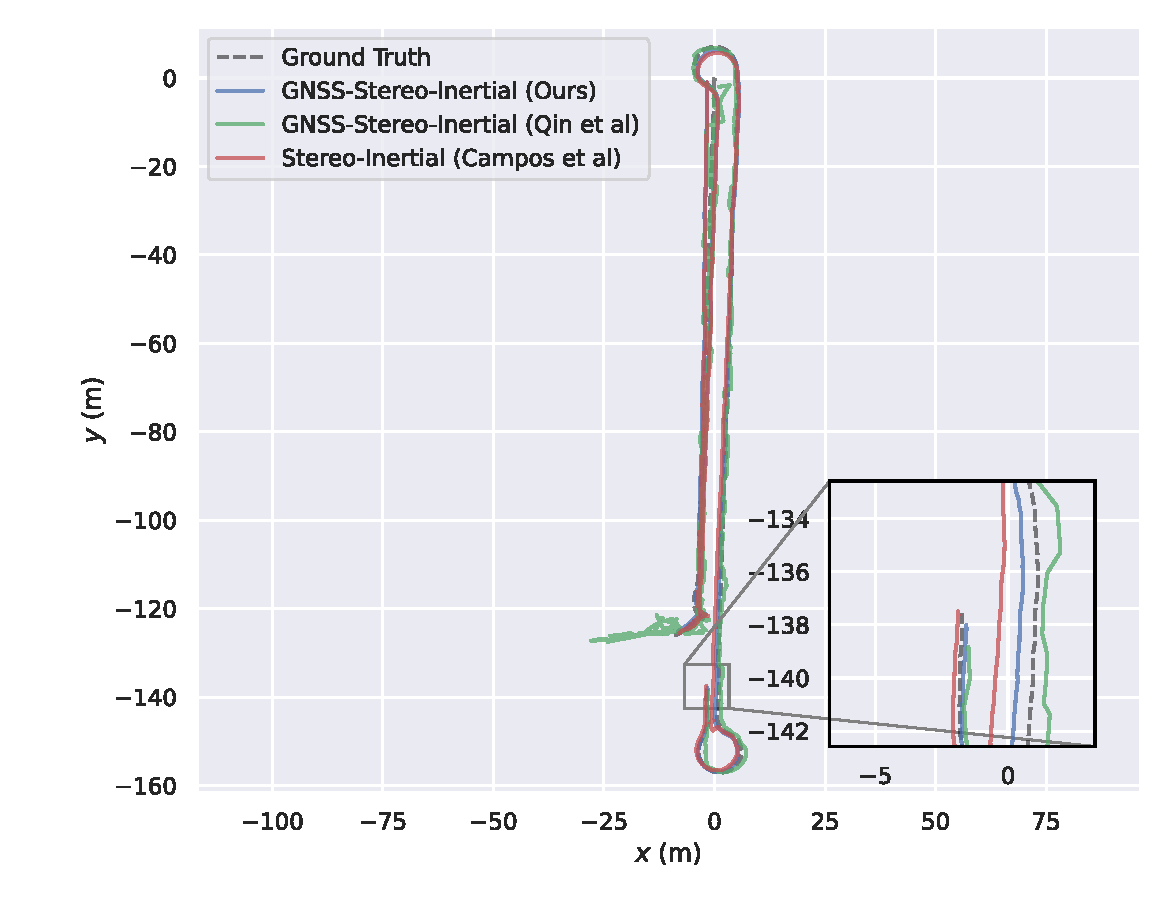
\includegraphics[width=0.42\textwidth]{images/seq01.pdf}}
  \hspace{1cm}
  \subfloat[Sequence 02\label{trajectories_sequence_02}]{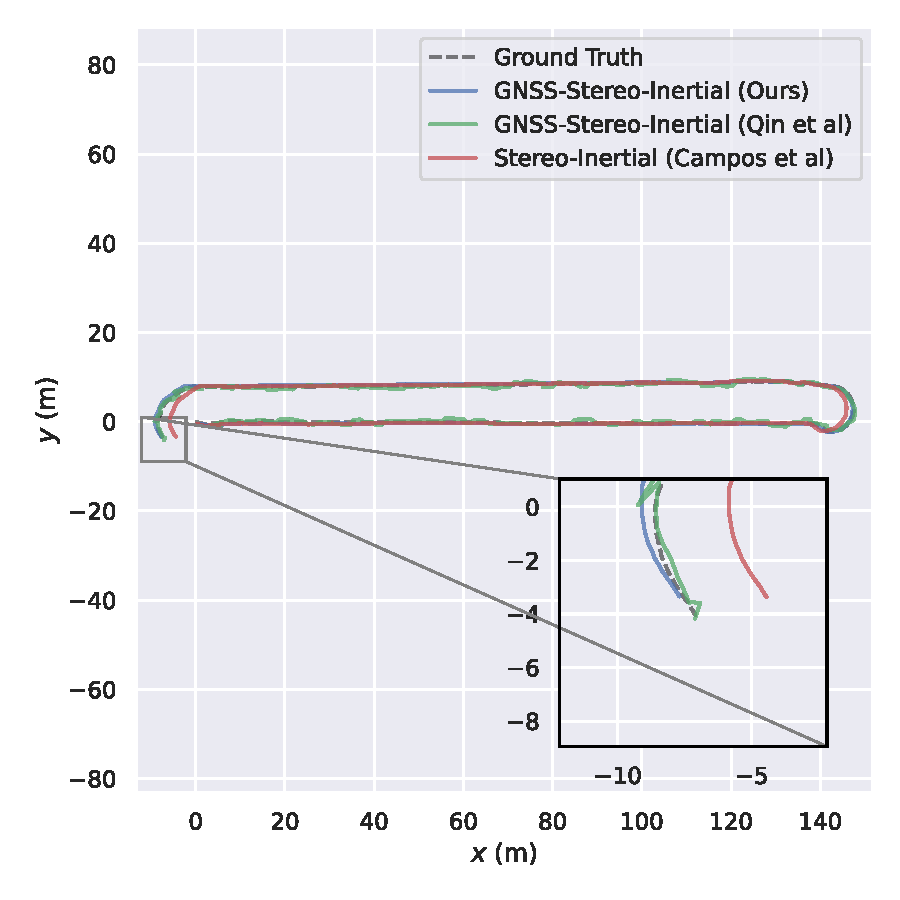
\includegraphics[width=0.42\textwidth]{images/seq02.pdf}\label{trajectories_sequence_02_int}}\\
  \subfloat[Sequence 03\label{trajectories_sequence_03}]{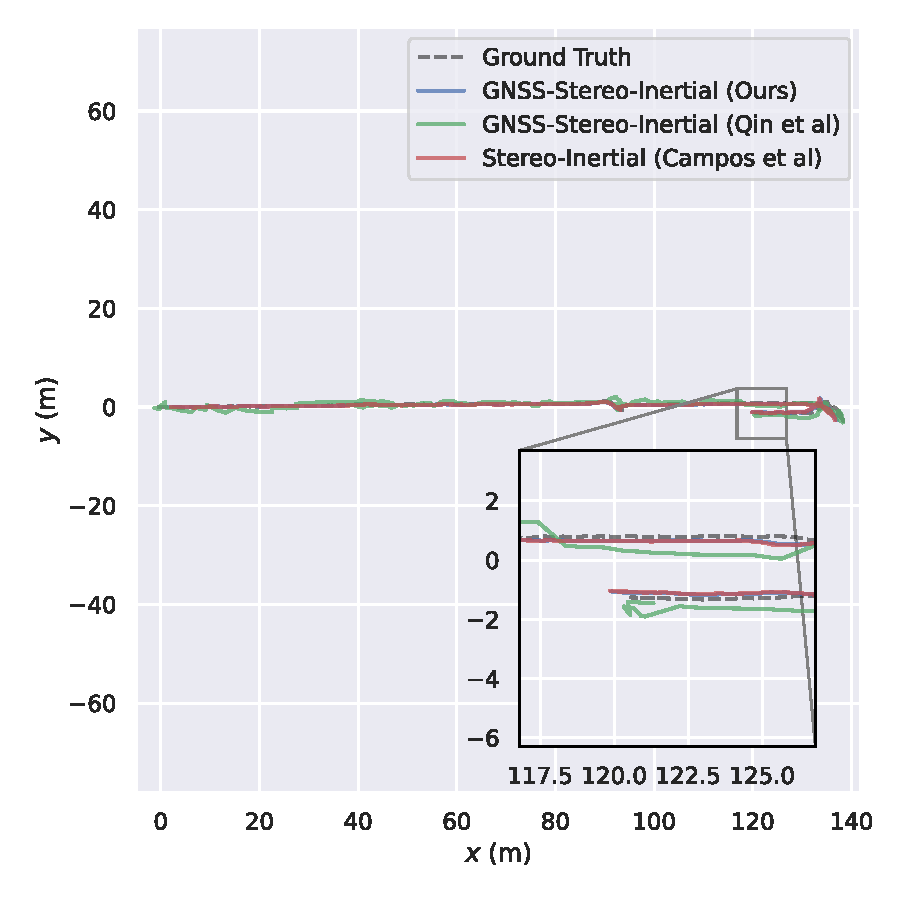
\includegraphics[width=0.42\textwidth]{images/seq03.pdf}}
  \hspace{1cm}
  \subfloat[Sequence 04\label{trajectories_sequence_04}]{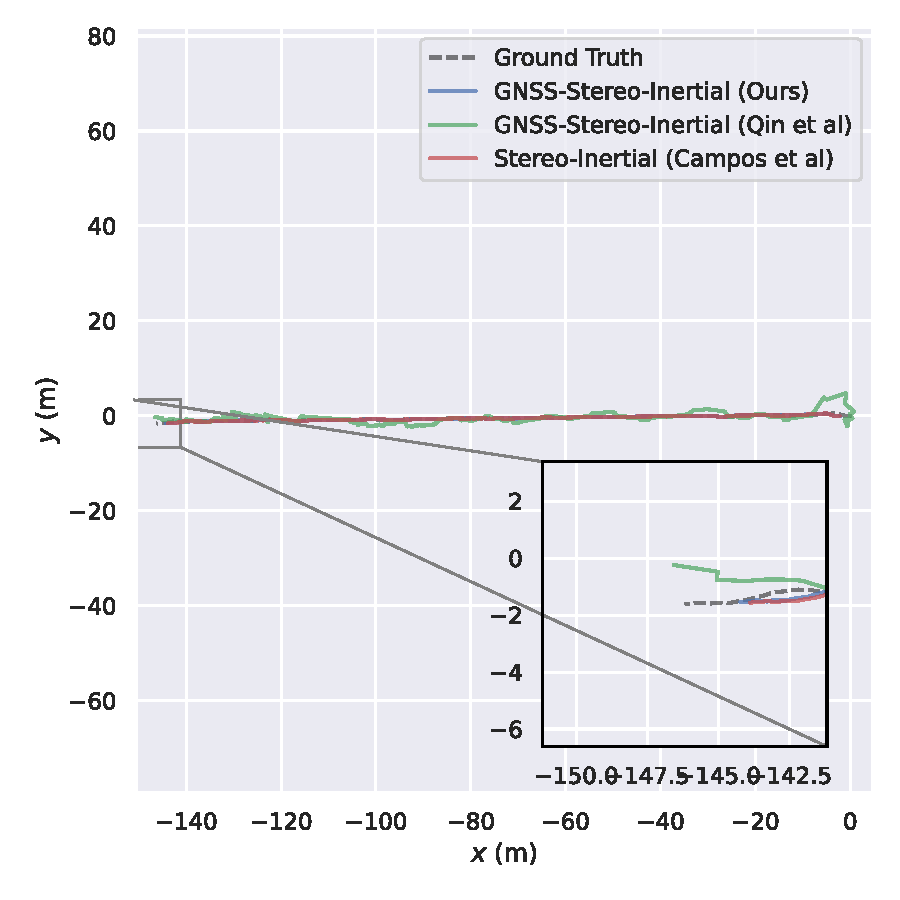
\includegraphics[width=0.42\textwidth]{images/seq04.pdf}}\\
  \subfloat[Sequence 05\label{trajectories_sequence_05}]{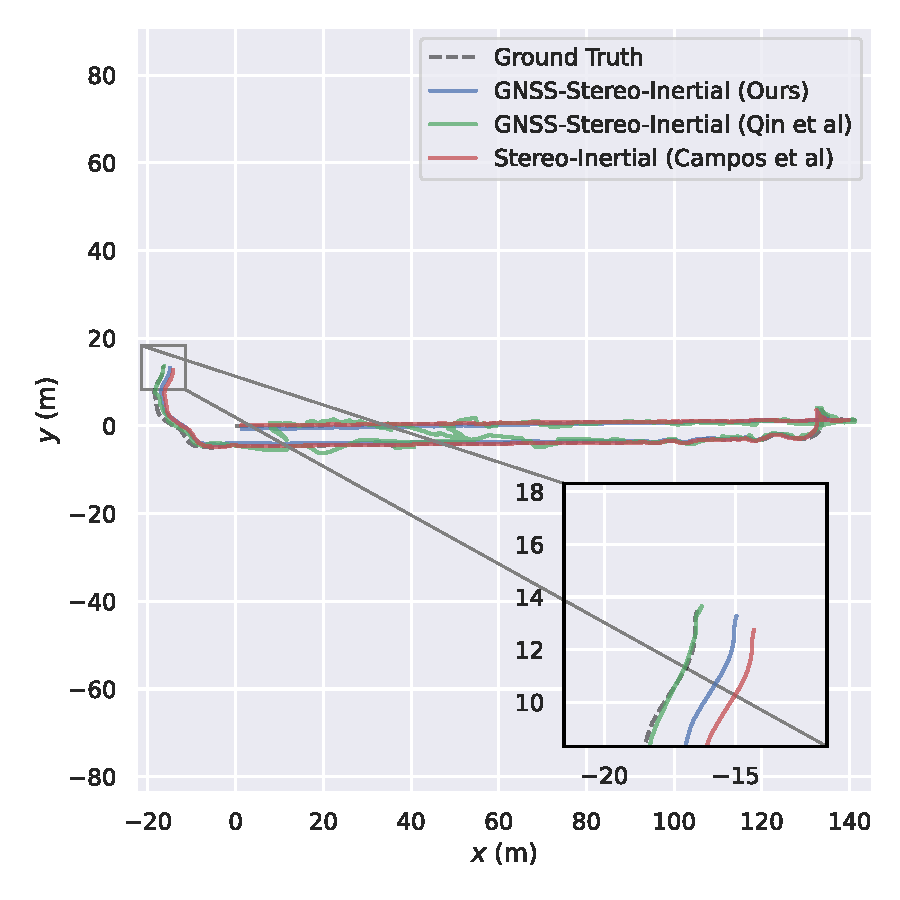
\includegraphics[width=0.42\textwidth]{images/seq05.pdf}}
  \hspace{1cm}
  \subfloat[Sequence 06\label{trajectories_sequence_06}]{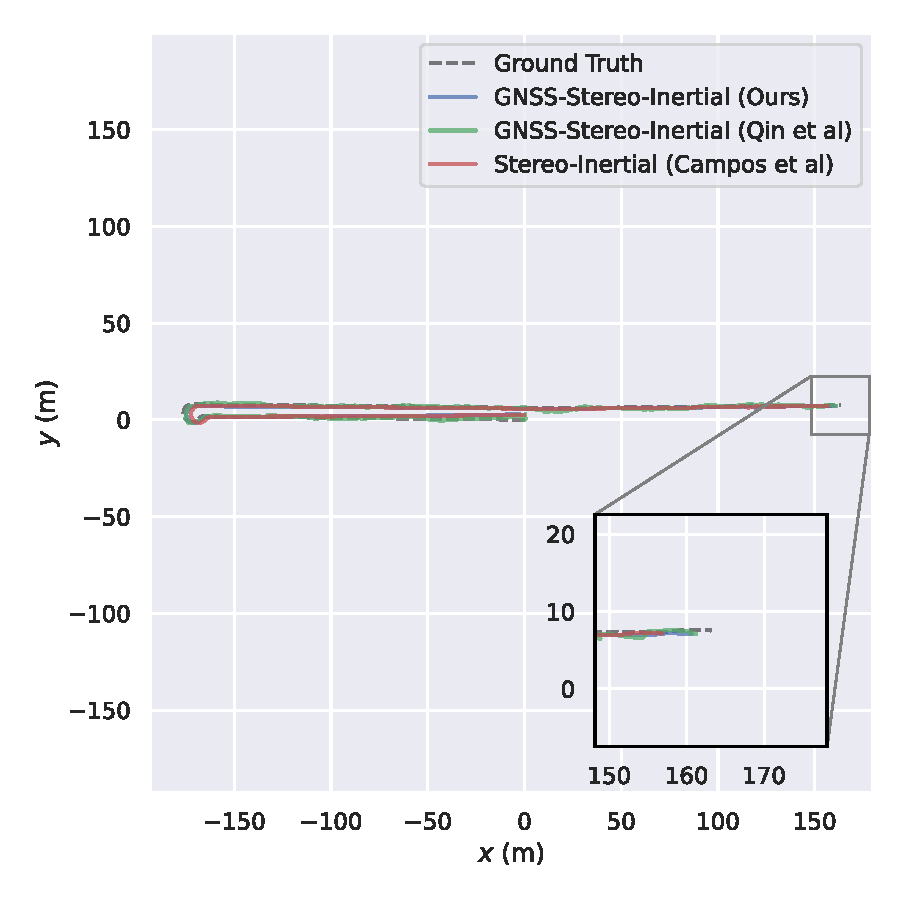
\includegraphics[width=0.42\textwidth]{images/seq06.pdf}}
  \caption{Results from Stereo-Inertial ORB-SLAM3 \cite{campos2021orbslam3}, a loosely-coupled GNSS-Stereo-Inertial system \cite{qin2019general} and our tightly-coupled GNSS-Stereo-Inertial system on the Rosario Dataset.}
  \label{fig:trajectories_rosario}
\end{figure*}

\subsection{Data with conventional GNSS in soybean fields}
\label{sec:experiments_conventional_gps}
In the experiments from the previous section, noisy GNSS measurements had to be simulated from GNSS-RTK ones, as the dataset does not contain conventional GNSS measurements. In this section we present an evaluation with conventional GNSS measurements. For this, we equipped our weed removal robot with such sensor and deployed it again in a soybean field. On board the robot there is a ZED stereo camera which captures images $\si{1280}\times\SI{720}{\px}$ at \SI{15}{\hertz}, an Emlid Reach GNSS operating at a frequency of \SI{5}{\hertz}, and an InvenSense MPU-9250 IMU set at \SI{200}{\hertz}. The covariance of the conventional GNSS measurements is offered by the driver of the GNSS receiver. In addition, there is an GNSS-RTK used as positional ground-truth. Figure~\ref{fig:robot} shows the robot configuration in the soybean field. We commanded the robot to record two data sequences. The corresponding GNSS-RTK trajectories are shown in Figure~\ref{fig:satellital} and images samples captured by the ZED camera can be seen in Figure~\ref{fig:image_samples}.

\begin{figure}[t]
    \centering
    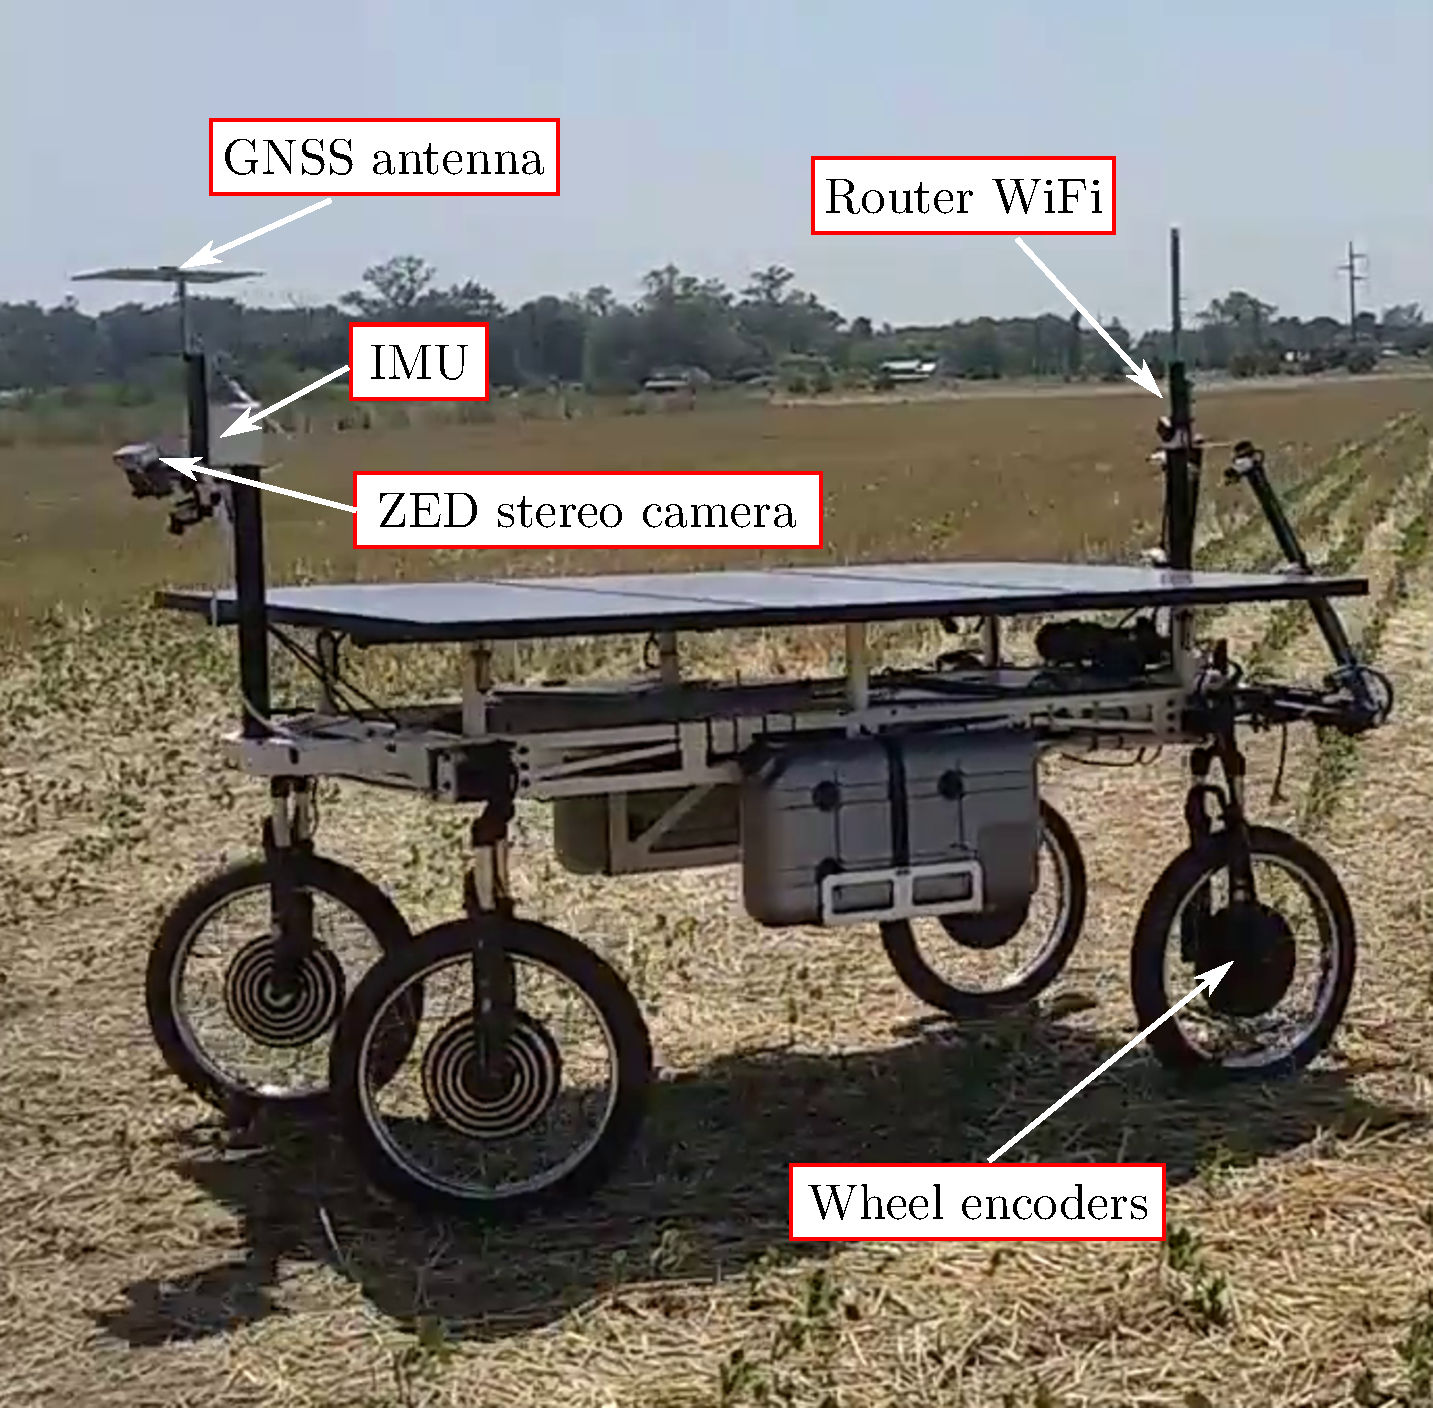
\includegraphics[width=\columnwidth]{images/robot_2022.pdf}
    \caption{Weed removal robot used in our in-house dataset in a soybean field.}
    \label{fig:robot}
\end{figure}

\begin{figure}[t]
    \centering
    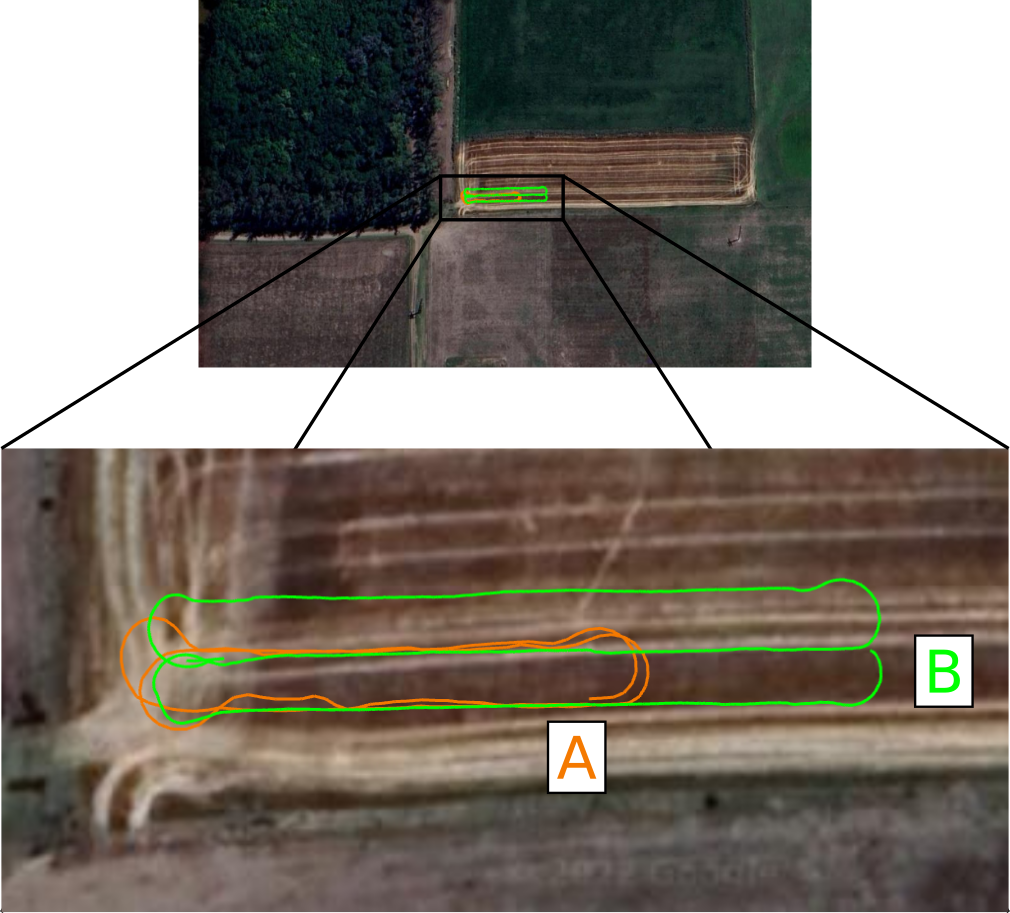
\includegraphics[width=\columnwidth]{images/satellital.png}
    \caption{GNSS-RTK trajectories for the sequences A (orange) and B (green) of the in-house recordings in the soybean field.}
    \label{fig:satellital}
\end{figure}

\begin{figure}[tp]
    \centering
    \subfloat{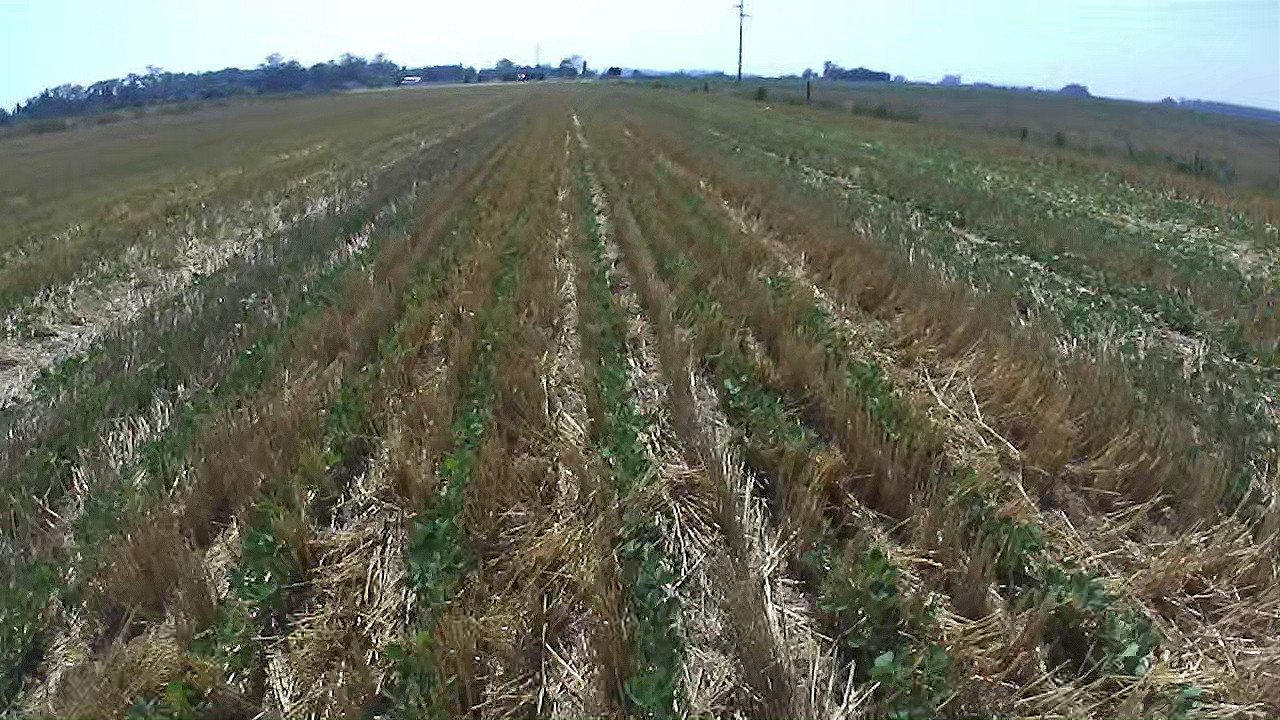
\includegraphics[width=0.45\columnwidth]{images/frame000000.jpg}}
    \hspace{0.1em}
    \subfloat{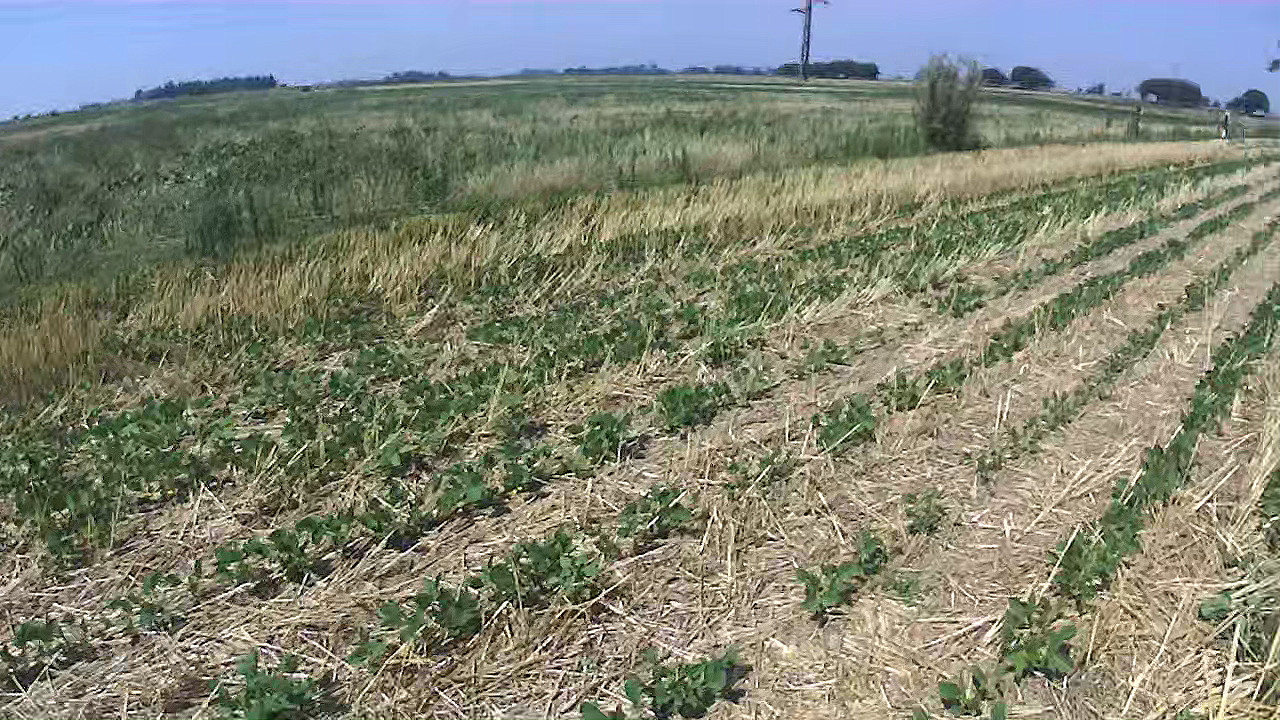
\includegraphics[width=0.45\columnwidth]{images/frame000136.jpg}}\\
    \subfloat{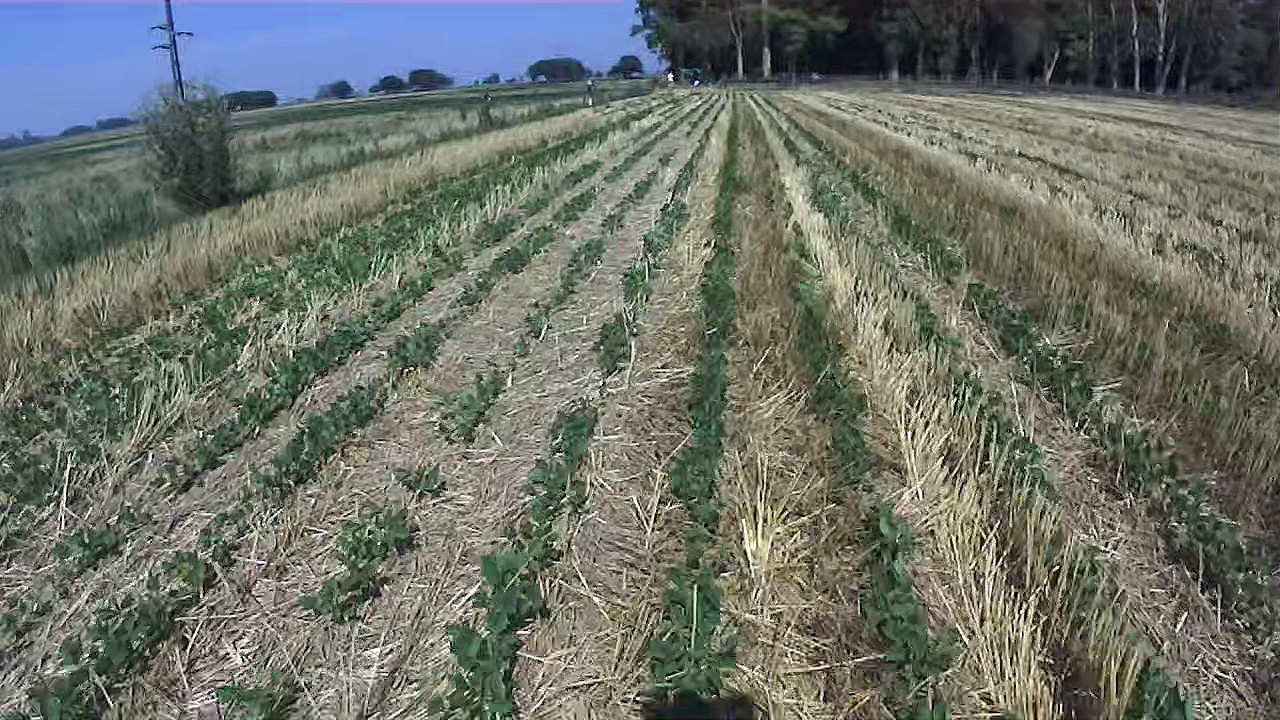
\includegraphics[width=0.45\columnwidth]{images/frame000200.jpg}}
    \hspace{0.1em}
    \subfloat{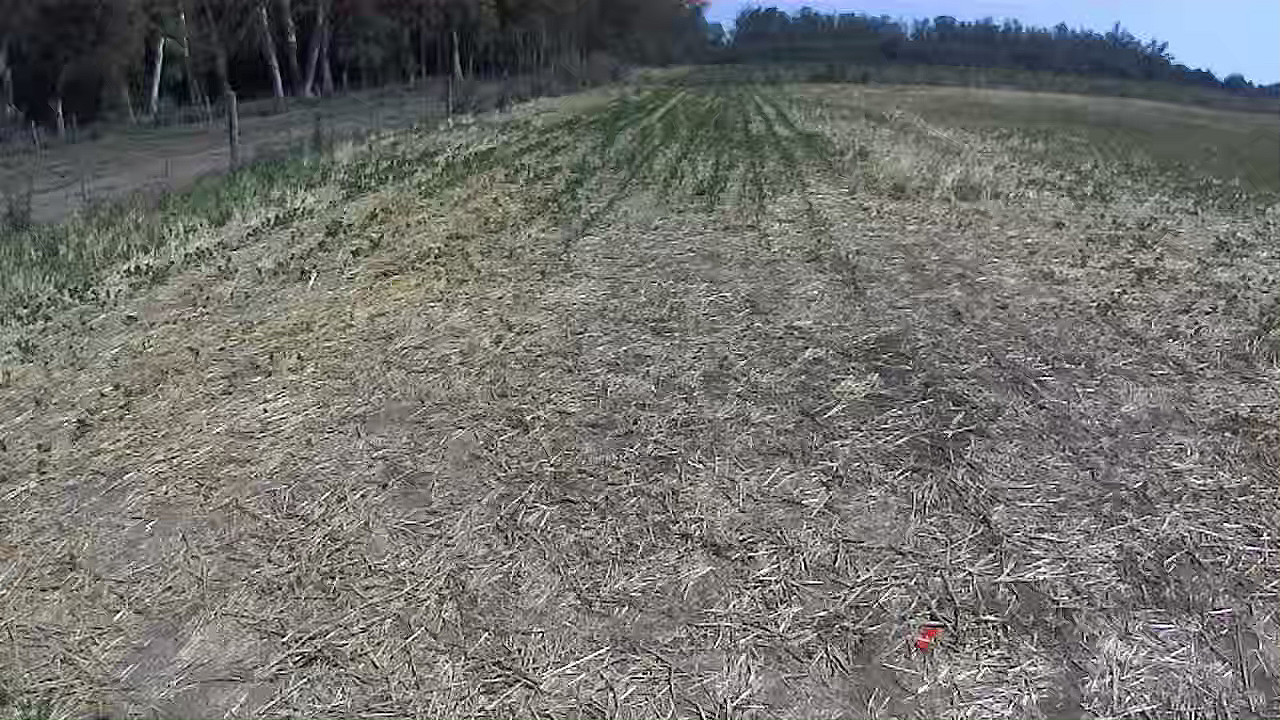
\includegraphics[width=0.45\columnwidth]{images/frame001264.jpg}}\\
    \subfloat{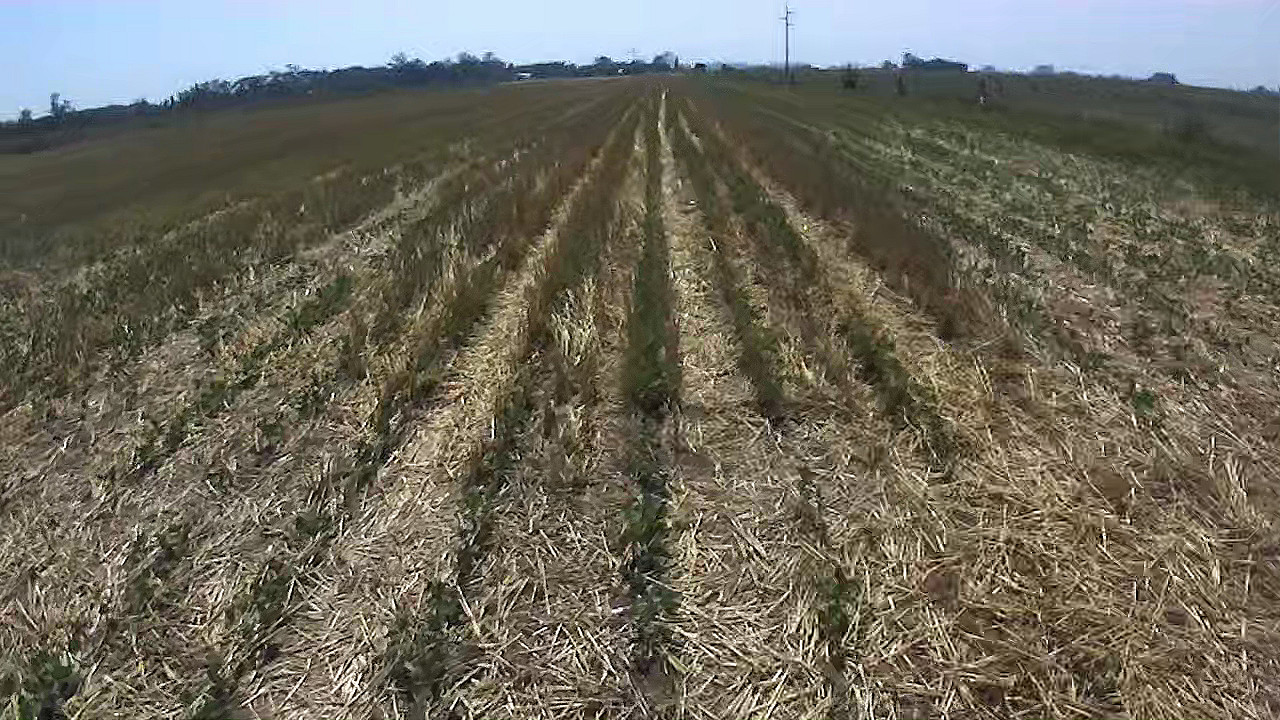
\includegraphics[width=0.45\columnwidth]{images/frame001364.jpg}}
    \hspace{0.1em}
    \subfloat{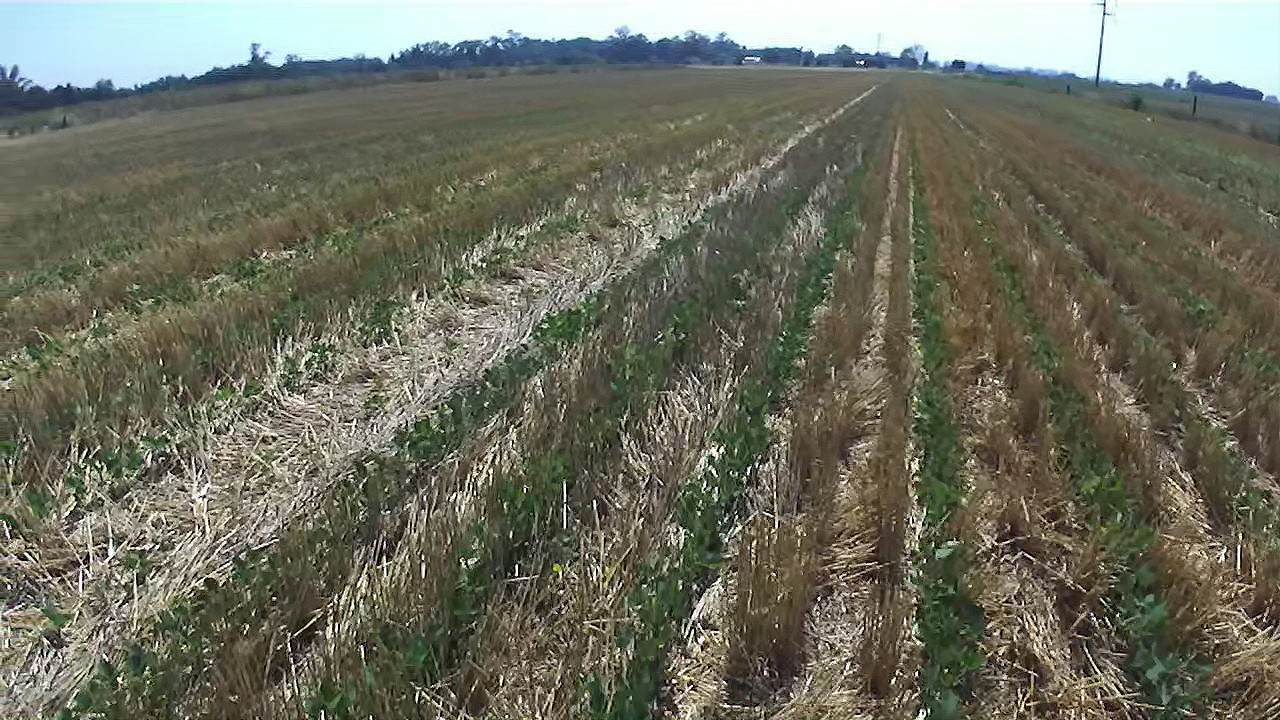
\includegraphics[width=0.45\columnwidth]{images/frame002477.jpg}}
    \caption{Sample images from our in-house dataset. Note the repetitive textures, a challenge for visual SLAM.}
    \label{fig:image_samples}
\end{figure}


On this data we ran the three frameworks mentioned in the previous experiment. The results of this experiment are shown in Table~\ref{tab:real_gps_results}, while the trajectories can be seen in the Figure~\ref{fig:trajectories_zavalla}. Estimated trajectories were aligned again with the ground-truth using
Umeyama's method.
\begin{table}[!tp]
    \centering
    \caption{Mean and standard deviation (between parentheses) of the Absolute Trajectory Error (ATE) [\si{\metre}] for stereo-inertial ORB-SLAM3 \cite{campos2021orbslam3}, a loosely-coupled GNSS-stereo-inertial system \cite{qin2019general} and our tightly-coupled GNSS-stereo-inertial framework in the in-house recordings in soybean fields. Best results are in \bf{bold}.}
    
    \resizebox{\linewidth}{!} {
        \begin{tabular}{cccc}
        \hline
                    Sequence & Stereo-Inertial & GNSS-Stereo-Inertial & GNSS-Stereo-Inertial \\
                    & \cite{campos2021orbslam3} & \cite{qin2019general} & (Ours) \\ \hline
        A &  0.64 (0.33) &  1.08 (0.78)                &  \bf{0.44 (0.16)} \\
        B & 0.43 (0.18)  &    5.58 (3.57)              & \bf{0.36 (0.13)} 
        \\
 \hline
        \end{tabular}
    }
    \label{tab:real_gps_results}
\end{table}

\begin{figure*}[!btp]
    \centering
    \subfloat[Sequence A\label{trajectories_sequence_A}]{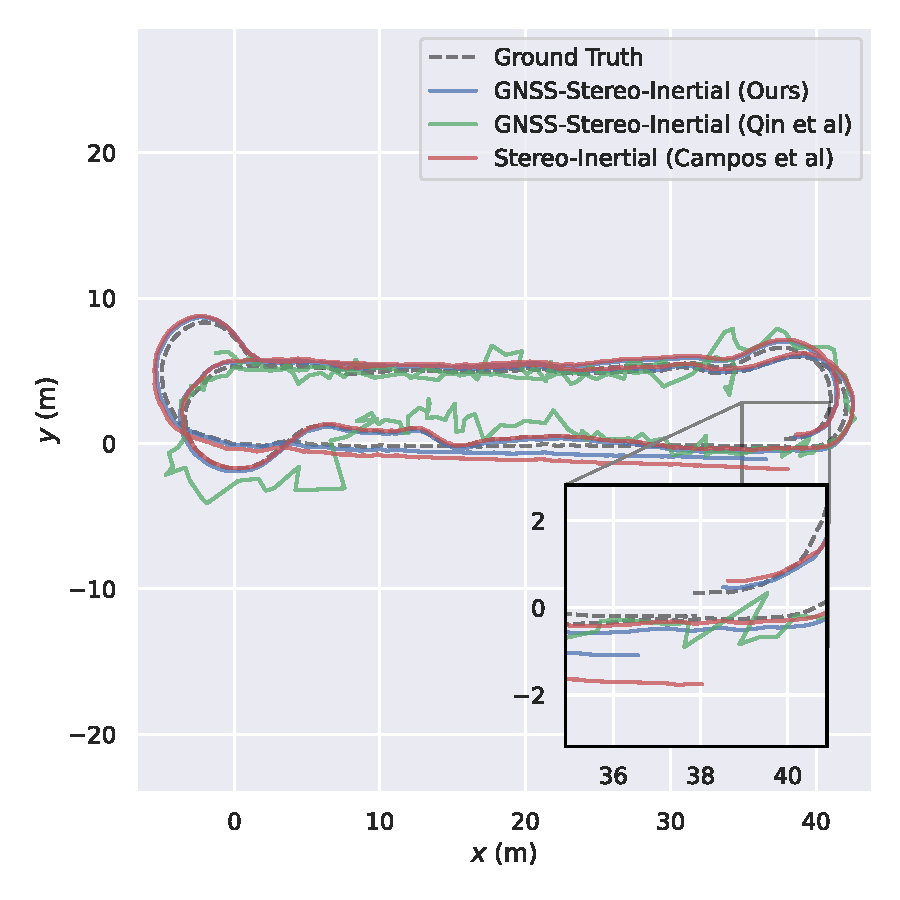
\includegraphics[width=0.42\textwidth]{images/zavalla_a.pdf}}
  \hspace{1cm}
  \subfloat[Sequence B\label{trajectories_sequence_B}]{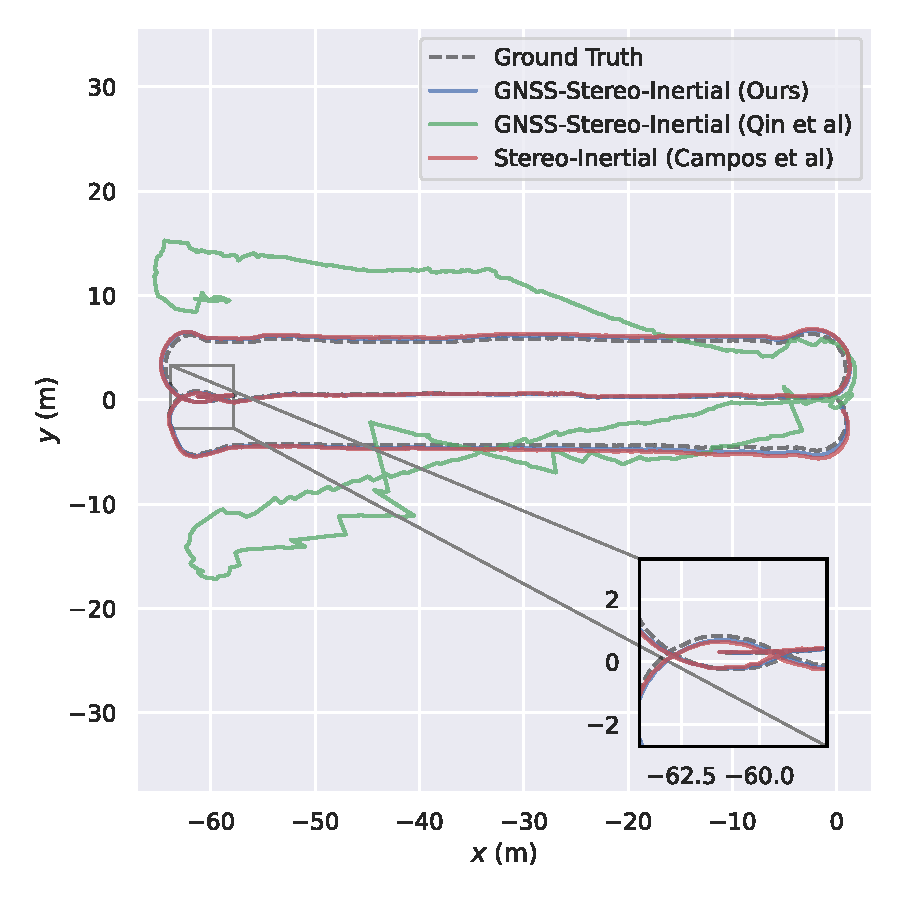
\includegraphics[width=0.42\textwidth]{images/zavalla_b.pdf}}\\
    \caption{Results from Stereo-Inertial ORB-SLAM3 \cite{campos2021orbslam3}, the loosely-coupled GNSS-Stereo-Inertial system of \cite{qin2019general} and our tightly-coupled GNSS-Stereo-Inertial implementation on our in-house recordings in soybean fields, using conventional GNSS. Note the smaller errors of tightly-coupled approaches, and how our GNSS fusion improves over the stereo-inertial baseline.}
    \label{fig:trajectories_zavalla}
\end{figure*}

\subsection{Discussion}
As can be seen in the results, our implementation clearly outperforms the stereo-inertial configuration of ORB-SLAM3 and the loosely-coupled approach in \cite{qin2019general}. As a very relevant note, we ran the full stereo-inertial ORB-SLAM3 in our configuration sequences with loop closure capabilities and, with its configuration by default, it was unable to detect previously visited locations and hence close loops due to insufficiently discriminative visual appearances of the agricultural environment (\emph{perceptual aliasing}). Although the default configuration for the loop closure parameters might be loosened to detect a higher number of loop closures, that would also produce a higher number of false positives (due again to perceptual aliasing) that would corrupt the estimation. These challenges are the main motivation for incorporating global positioning sensors in agricultural environments, allowing to reduce the drift without depending on visual features. Very interestingly, we found in our experiments that only one third of the optimized keyframes had associated GNSS measurements. This may indicate that high-frequency GNSS measurements are not necessary to improve the estimation of visual-inertial SLAM, and a sparse subset of them might suffice to offer a reasonable performance.

Unlike the loosely-coupled system, our implementation returns smoother trajectories. Moreover, since the fusion is loosely-coupled, the global position measurements correct the estimate without considering the continuous motion of the robot and acts as an interpolation between the underlying visual-inertial system and the GNSS measurement. Even though in sequence 02 of the Rosario Dataset, the loosely-coupled fusion system obtains a lower error, in the trajectory of the Figure~\ref{fig:trajectories_rosario} it can be observed that the estimation looks bumpy. Smooth pose estimation, like the one offered by our tightly-coupled approach, is more suitable for use in a navigation control algorithm.

Regarding the experiment with conventional GNSS measurements, it should be pointed out that the loosely-coupled system lost the visual-inertial tracking in the two sequences. This indicates that it is important not only to focus on global measurements, but also to have a robust visual-inertial fusion. In our case, we use ORB-SLAM3 as the underlying system, as a result of having analyzed the performance of different visual-inertial systems in previous research \cite{cremona2022evaluation}. As a conclusion, in addition to a tight coupling of the sensor data, the robustness of the visual-inertial estimates are also relevant for practical implementations in agricultural applications.

An important consideration is the modelling of the noise of GNSS measurements. Based on previous works \cite{cioffi2020tightly, boche2022dropout}, the uncertainty was modelled as additive isotropic Gaussian noise. This is a simple model that arises naturally from the GNSS device data, as the device drivers generally provide a covariance of the position. Other ways of modelling the noise of GNSS measurements in the context of pose estimation are worth studying, as when comparing the simulated signal in the section \ref{sec:experiments_rosario_dataset} experiment with the conventional GNSS signal used in the field experiments, differences in their behaviour were observed. When the conventional GNSS signal was inspected in detail, a bias was found, mainly at altitude, which could be verified by the GNSS-RTK. Therefore, this topic should be addressed in future work.


\section{Conclusion}
\label{sec:conclusion}
\section{Conclusion} \label{conclusion}

The preliminary design of the Dragonfly navigation filter has been developed and demonstrated to robustly navigate the vehicle over multiple kilometer flights in a high fidelity Titan simulation. While the Dragonfly mission is unique, several contributions are applicable to the broader inertial navigation, VIO, and TRN fields including a new architecture for redundant IMUs, improving global heading and position knowledge by revisiting images after re-initializing the filter on the surface, and a robust approximation to the SLAM formulation. Several updates and optimizations are underway to improve the nav filter including porting the EKF to the UDU implementation~\cite{carpenter2018}, modeling correlated pressure sensor measurements, reducing the nav filter update rate to 1 Hz, and a higher fidelity terrain model. An alternate breadcrumb model is also being explored to better preserve cross covariance information with all the filter states. Filter updates to support image processing updates are also expected in the next phase, such as using processing multiple image patches or ingesting the displacement measurement directly in pixels.  

\clearpage
{\small
% \bibliographystyle{unsrt}
\bibliographystyle{ieee_fullname}
\bibliography{egbib}
}

\end{document}